% -*- program: xelatex -*-
%\documentclass[12pt, compress]{beamer} 
\documentclass[11pt, compress]{beamer}       
%\documentclass[notes=only]{beamer}

\usepackage{fontspec}
	
\setsansfont{PT Sans}
 \setmonofont{Liberation Mono}

\usepackage{beamerthemesplit}
\usefonttheme[onlymath]{serif}
%\DeclareFontEncoding{T1}
\fontencoding{T1}

%\usepackage[T2A]{fontenc} 
\usepackage[utf8x]{inputenc}
\usepackage[russian]{babel}
\usepackage{listings}

\usepackage{amsmath,amssymb,amsthm}
\hypersetup{unicode=true}
\usepackage{graphics,graphicx}
\usepackage{verbatim}
\usepackage{fancyvrb}
\usepackage{booktabs} 
%\usepackage{media9}
\usepackage[super]{natbib}
\usepackage{color}
\definecolor{mygreen}{RGB}{28,172,0} % color values Red, Green, Blue
\definecolor{mylilas}{RGB}{170,55,241}
\definecolor{codecolor}{RGB}{0,120,0}
\definecolor{light-gray}{gray}{0.95}
\definecolor{light-green}{rgb}{0.93, 1, 0.8}
\definecolor{light-yellow}{rgb}{1,1,0.85}
\definecolor{dark-blue}{rgb}{0,0,0.6}
\definecolor{dark-red}{rgb}{0.7,0,0.0}
\definecolor{dark-green}{RGB}{10,150,0}

\usepackage{pifont}% http://ctan.org/pkg/pifont
\newcommand{\cmark}{\textcolor{green}{\ding{51}}}
\newcommand{\xmark}{\textcolor{red}{\ding{55}}}

\setbeamercolor{frametitle}{fg=dark-red,bg=gray!10}
\setbeamerfont{title}{series=\bfseries,parent=structure}
\setbeamerfont{frametitle}{series=\bfseries,parent=structure}

\setbeamertemplate{blocks}[rounded][shadow=false]
\setbeamertemplate{navigation symbols}{}

\newcommand{\code}[1]{\textcolor{dark-green}{\texttt{#1}}}
\newcommand{\cleartitlepage}[1]{\begin{frame}[plain]\begin{center}\textsc{#1}\end{center}\end{frame}}
\renewcommand{\emph}[1]{\textcolor{dark-blue}{#1}}
\newcommand{\emphb}[1]{\textcolor{dark-blue}{\textbf{#1}}}
\newcommand{\lstcomment}[1]{\textcolor{dark-green}{\# \texttt{#1}}}

\usepackage{dirtree}
\usepackage{menukeys}

\usetheme{CambridgeUS}
\usecolortheme{lily}


\lstset{basicstyle=\ttfamily,
    numbers=none,
    language=gnuplot,    
    keepspaces=true,
    extendedchars=\true,
    basicstyle={\small},
    breaklines=true, 
    morekeywords={matlab2tikz},
    keywordstyle=\color{blue},
    morekeywords=[2]{1}, keywordstyle=[2]{\color{blue}},
    identifierstyle={ \bf \color{black} },
    stringstyle=\color{mylilas},
    commentstyle=\color{mygreen},%
    showstringspaces=false,
    numbers=left,%
    numberstyle={\scriptsize \color{gray}},
    numbersep=7pt, 
    emph=[1]{colorspace,convert,resize,density,geometry,bordercolor,montage,tile,ffmpeg},emphstyle=[1]\color{blue}, 
    frame=single,    
    rulecolor=\color{red},    
    backgroundcolor=\color{light-gray},
    xleftmargin=0.3cm,
    frame=l,framesep=4pt,framerule=0.5pt,
    escapechar=|
    %lineskip=-1.0pt,
    %emph=[2]{word1,word2}, emphstyle=[2]{style},    
}

\usepackage{tikz}
\usetikzlibrary{calc,patterns,decorations.pathmorphing,decorations.markings,positioning}
\tikzset{cbutton/.style={rectangle,minimum width=10mm,thick,draw=red!50!black!50,
top color=white,bottom color=red!50!black!30}}
\tikzset{mbutton/.style={rectangle,minimum width=10mm,thick,draw=black!20,
top color=white,bottom color=black!30}}

\usetikzlibrary{arrows,shapes}
\tikzstyle{every picture}+=[remember picture]


\makeatother
\setbeamertemplate{footline}
{
  \leavevmode%
  \hbox{%  
  \begin{beamercolorbox}[wd=.3\paperwidth,ht=2.25ex,dp=1ex,center]{author in head/foot}%
    \usebeamerfont{author in head/foot}\insertshortauthor
  \end{beamercolorbox}%  
  \begin{beamercolorbox}[wd=.6\paperwidth,ht=2.25ex,dp=1ex,center]{title in head/foot}%
    \usebeamerfont{title in head/foot}\insertshorttitle
  \end{beamercolorbox}%
  \begin{beamercolorbox}[wd=.1\paperwidth,ht=2.25ex,dp=1ex,center]{date in head/foot}%
    \insertframenumber{} / \inserttotalframenumber\hspace*{1ex}
  \end{beamercolorbox}}%
  \vskip0pt%
}

\setbeamertemplate{headline}{}
\setbeamertemplate{footline}{}
 
\AtBeginSection[]{
  \begin{frame}[plain]
  %\vfill  
  \begin{tikzpicture}
  \useasboundingbox (0,0) rectangle(\the\paperwidth,\the\paperheight);  
  \fill[color=dark-red]   (-1cm, 3.9cm) rectangle(\the\paperwidth, 5.9cm);
  %\usebeamerfont{title}\insertsectionhead\par%
  %\node[text width=\the\paperwidth,align=center] at (current page.center) {\color{ExecusharesWhite}\Large\textbf{\insertsectionhead}};  
  \node[text width=\the\paperwidth,align=center] at (6cm,4.9cm) {\color{white}\Large\textbf{\insertsectionhead}};  
  \end{tikzpicture}
  \end{frame}
}


\graphicspath{{./img/}}

% ============================================================================

\title{ImageMagick \& ffmpeg}
\subtitle{Компьютерная графика}
\author[Самарский университет]{Юдинцев В. В.}
\institute{Кафедра теоретической механики}
\date{\today}

\usepackage{tikz}
\usetikzlibrary{positioning} 
\tikzset{cbutton/.style={rectangle,minimum width=10mm,thick,draw=red!50!black!50,
top color=white,bottom color=red!50!black!30}}
\tikzset{mbutton/.style={rectangle,minimum width=10mm,thick,draw=black!20,
top color=white,bottom color=black!30}}


\tikzstyle{block} = [rectangle, draw, fill=yellow!20, text width=5em, text centered, rounded corners, minimum height=5em]
\tikzstyle{subblock} = [rectangle, draw, fill=white, text width=2em, text centered, minimum height=1em]
\tikzstyle{module} = [rectangle, draw, fill=none, text width=5em, text centered, rounded corners, minimum height=5em]
\tikzstyle{line} = [draw, ->]

\begin{document}

{
\setbeamercolor{background canvas}{bg=light-yellow} 
\usebackgroundtemplate{
\includegraphics[width=\paperwidth,height=\paperheight]{back.png}}
\begin{frame}[plain]
%\begin{figure}[h]
%  \centering
%  \includegraphics[width=0.3\textwidth]{../common/Python_logo_and_wordmark.pdf}
%\end{figure}
\maketitle
\end{frame}
}

\frame{\frametitle{Содержание}\tableofcontents}

\section{Работа с командной строкой}

\begin{frame}[c, fragile]
\frametitle{Командная строка}
Открыть командную строку в текущем каталоге проводника: \keys{Shift}+\keys{ПКМ}  
\begin{center}
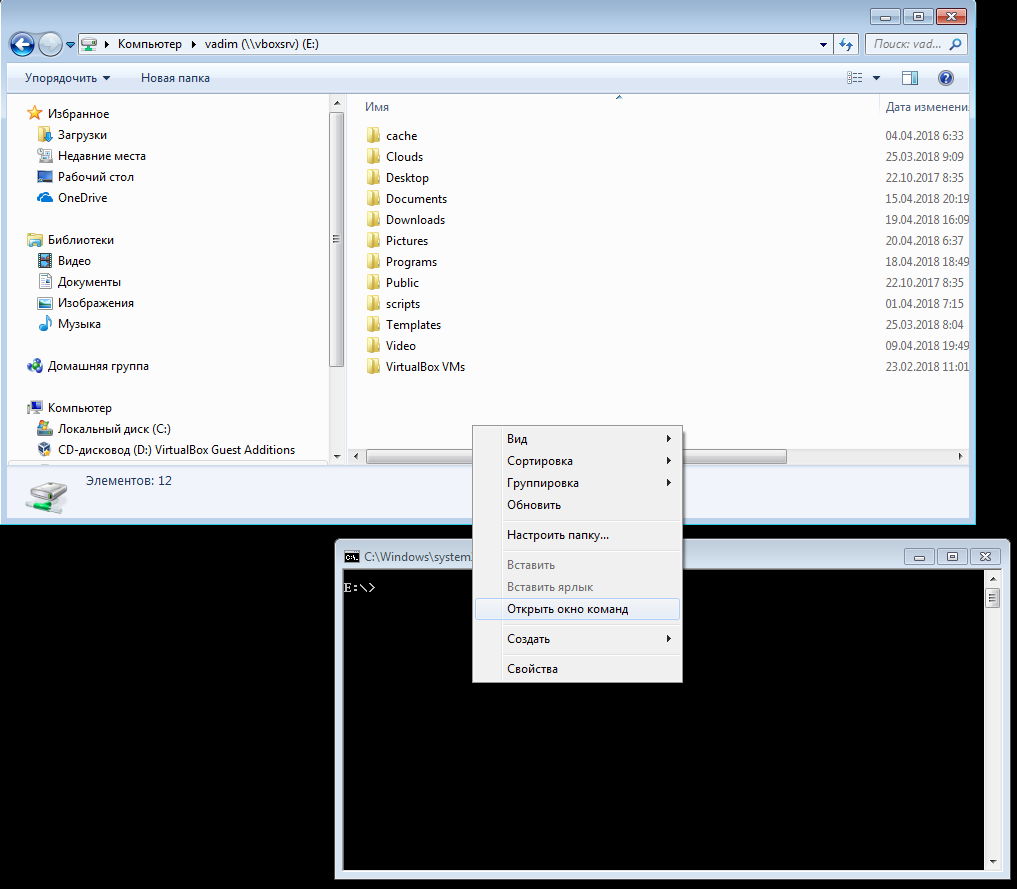
\includegraphics[width=0.6\textwidth]{cmd.png}
\end{center}
\end{frame} 


\section{ImageMagick}

\begin{frame}[c, fragile]
\begin{itemize}
   \item \emph{ImageMagick} -- набор программ командной строки для преобразования, создания графических файлов.
   \item \emph{ImageMagick} поддерживает около 200 форматов файлов.   
\end{itemize} 
\end{frame}

\begin{frame}[c, fragile]
\frametitle{Основные утилиты}
\begin{itemize}
	\item \emph{convert} -- преобразование
	\item \emph{mogrify} -- преобразование с заменой исходного файла (файлов)
  \item \emph{montage} -- монтаж
	\item \emph{compose} -- совмещение (композиция) изображений
\end{itemize}
\end{frame}

\begin{frame}[t]
\frametitle{Установка}
{\small \url{https://www.imagemagick.org/script/download.php\#windows}}
\begin{figure}[htbp]
\centering
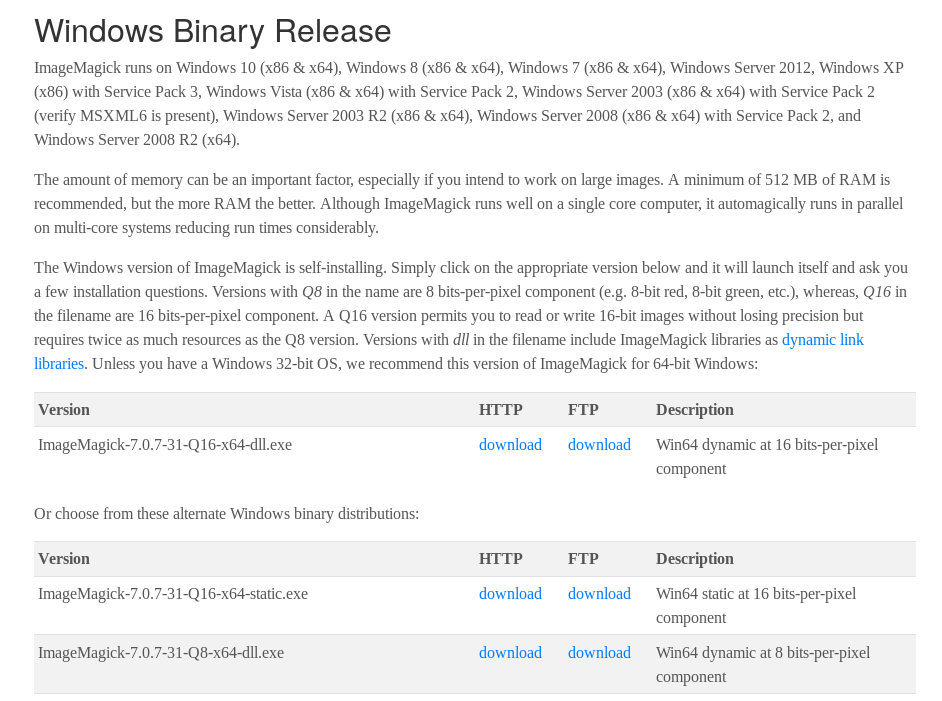
\includegraphics[width=0.95\textwidth]{imagemagick.png}
\end{figure}
  
\end{frame}

\begin{frame}[c, fragile]
\frametitle{Преобразование типов файлов}
Программа (утилита) \emph{convert} может использоваться для преобразования форматов графических файлов. 
\begin{itemize}
\item преобразование изображения формата \emph{.png} в формат \emph{.jpg}:
\begin{lstlisting}
convert myPhoto.png myPhoto.jpg
\end{lstlisting}
\item при преобразовании в формат, предполагающий потерю качества (\emph{.jpg}) можно указать степень сжатия: 
\begin{lstlisting}
convert myPhoto.png -quality 10 myPhoto.jpg
\end{lstlisting}
для формата jpg это число обычно не ниже 75.
\end{itemize}
\end{frame}

\begin{frame}[c]
\frametitle{Качество}
\begin{columns}
\column{0.5\linewidth}
Исходное изображение
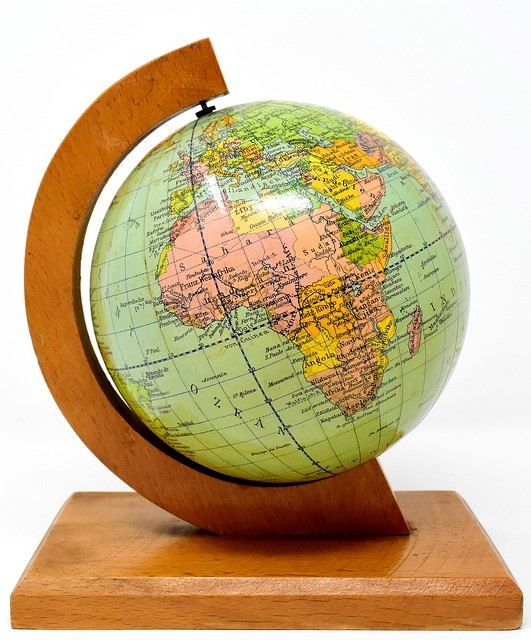
\includegraphics[width=0.95\textwidth]{globe.jpg}\\
102 Кб
\column{0.5\linewidth}
Качество (сжатие) 10\%
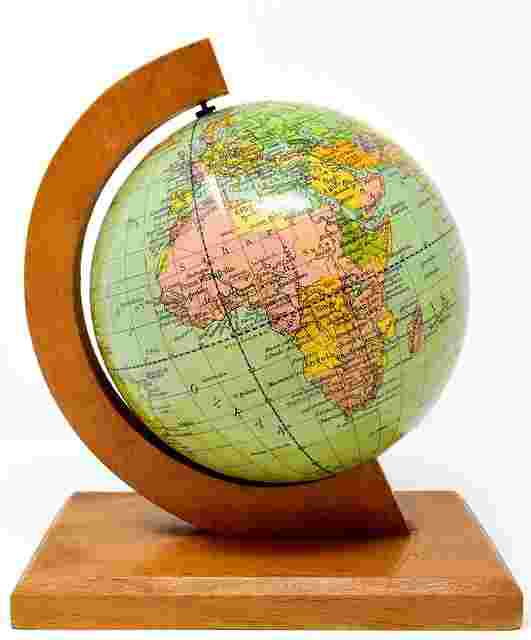
\includegraphics[width=0.95\textwidth]{globe10.jpg}\\ 
12 Кб
\end{columns}  
\end{frame}


\begin{frame}[c, fragile]
\frametitle{Преобразование из векторный форматов}
\begin{itemize}
\item Утилита \emph{convert} может использоваться для преобразования векторных форматов (pdf, svg, eps, ps) в растровый. 
\item В этом случае указывается качество детализации получаемого растрового изображения в точках на дюйм при помощи свойства \emph{-density}:
\item В результате преобразования pdf в jpg
\begin{lstlisting}
convert -density 300 Document.pdf Document.jpg
\end{lstlisting}
в каталоге появятся файлы Document-0.jpg, Document-1.jpg, ... Document-NN.jpg, где 'NN' -- количество страниц в документе.
\end{itemize}
\end{frame}

\begin{frame}[c, fragile]
\frametitle{Преобразование из векторный форматов}
\begin{columns}
\column{0.5\linewidth}
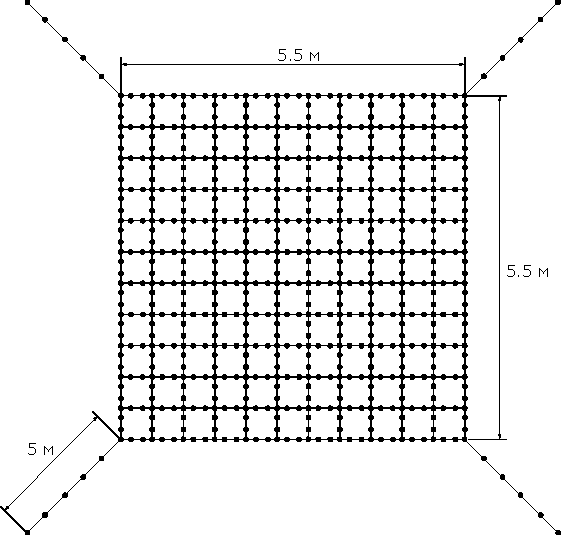
\includegraphics[width=0.95\textwidth]{net.pdf}
\column{0.5\linewidth}
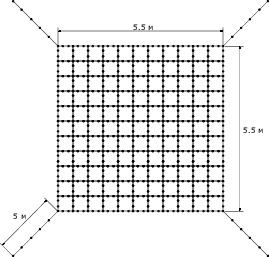
\includegraphics[width=0.95\textwidth]{net.jpg}
\end{columns}  
\vfill
\begin{lstlisting}
convert Document.pdf -flatten -background white 
        Document.jpg
\end{lstlisting}
\end{frame}

\begin{frame}[c, fragile]
\frametitle{Преобразование из векторный форматов}
\begin{columns}
\column{0.5\linewidth}
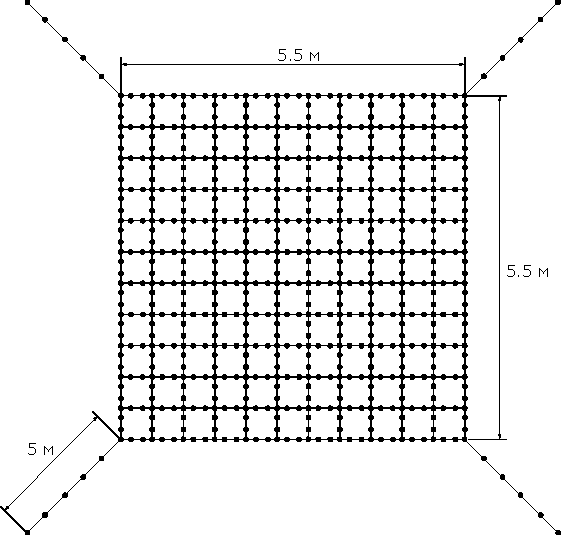
\includegraphics[width=0.95\textwidth]{net.pdf}
\column{0.5\linewidth}
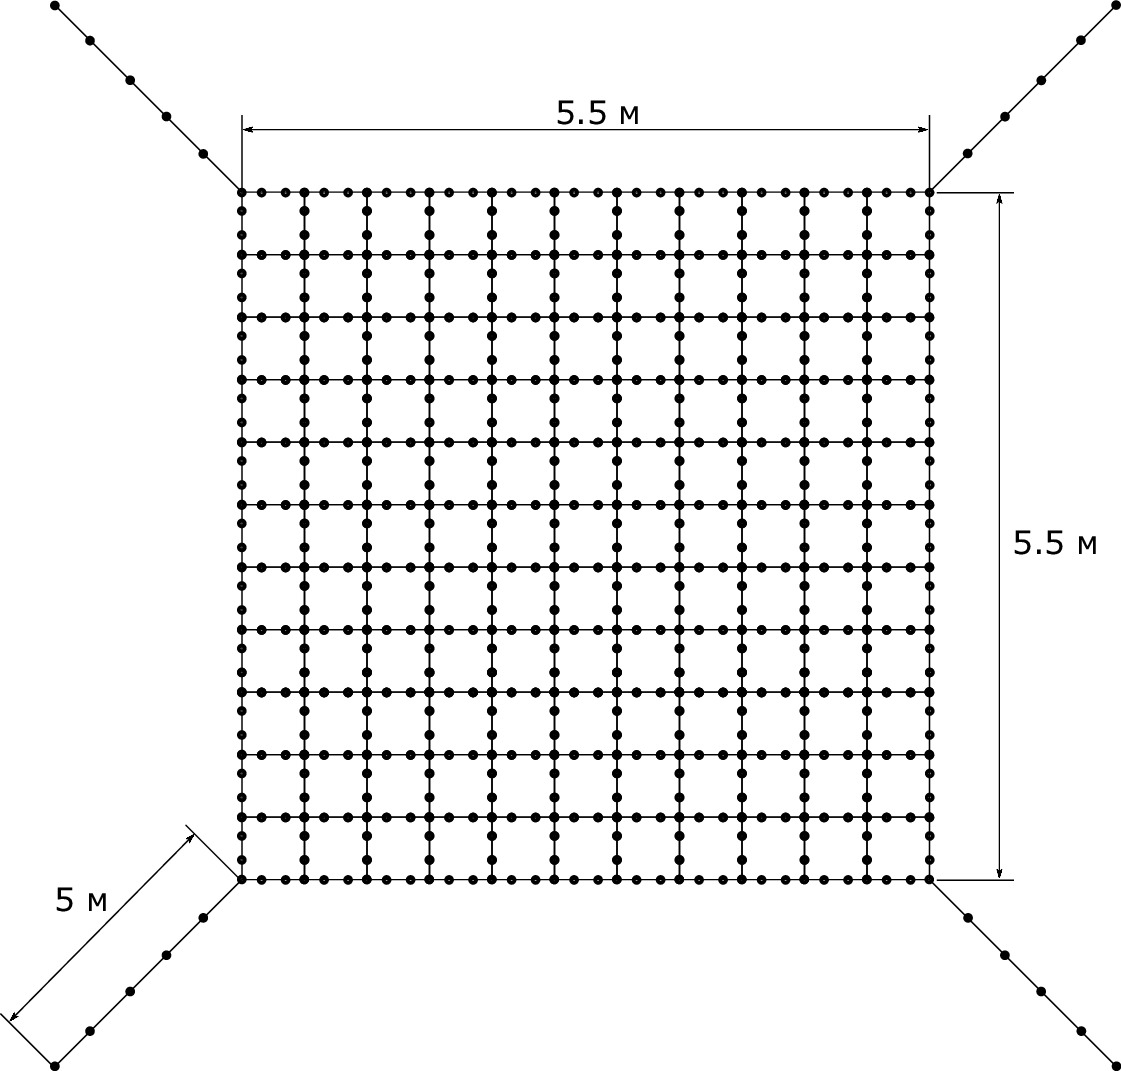
\includegraphics[width=0.95\textwidth]{net300.jpg}
\end{columns}  
\vfill
\begin{lstlisting}
convert -density 300 Document.pdf -flatten 
        -background white Document.jpg
\end{lstlisting}
\end{frame}

\begin{frame}[c, fragile]
\frametitle{Извлечение одной или нескольких страниц}
\begin{itemize}
\item Извлечение только первой страницы из документа \emph{pdf}:
\begin{lstlisting}
convert -density 300 document.pdf[0] image.jpg
\end{lstlisting}
\item Извлечение первых десяти страниц:
\begin{lstlisting}
convert -density 300 document.pdf[0-9] image.jpg
\end{lstlisting}
image-1.jpg, image-2.jpg, image-3.jpg, ... , image-9.jpg 
\item Извлечение первых десяти страниц (с указанием формата номера файлов-результатов):
\begin{lstlisting}
convert -density 300 doc.pdf[0-9] image_%02d.jpg
\end{lstlisting}
image\_01.jpg, image\_02.jpg, image\_03.jpg, ... , image\_09.jpg 
\end{itemize}
\end{frame}


\begin{frame}[c, fragile]
\frametitle{Преобразование формата}
\begin{itemize}
\item Преобразование формата с перезаписью исходного файла выполняется при помощи программы \code{mogryfi}
\begin{lstlisting}
mogrify  -format  jpg  image.png
\end{lstlisting}  
Файл \emph{image.png} преобразуется в формат \emph{jpg}. \alert{Исходный файл удаляется!}
\item Преобразование всех файлов формата \emph{.png} в текущем каталоге в формат \emph{.jpg}:
\begin{lstlisting}
mogrify  -format  jpg  *.png
\end{lstlisting}  
\end{itemize}
\end{frame}


\begin{frame}[c, fragile]
\frametitle{Изображения в pdf}
Программа \emph{convert} может использоваться для преобразования растровых форматов, например, отсканированных страниц, в многостраничный формат pdf:
\begin{itemize}
\item Все изображения формата jpg  в текущем каталоге преобразуются в многостраничный формат PDF
\begin{lstlisting}
convert *.jpg Document.pdf
\end{lstlisting}
\end{itemize}
\end{frame}

\begin{frame}[c, fragile]
\frametitle{Размер изображения}
\begin{itemize}
	\item Уменьшение изображения на 50\%:
\begin{lstlisting}
convert original.jpg -resize 50% small_50p.png
\end{lstlisting}
	\item Изменение размеров с указанием ширины и высоты (изображение вписывается в заданный прямоугольник): 
\begin{lstlisting}
convert original.jpg -resize 500x800 img500x800.png
\end{lstlisting}
\end{itemize}
\end{frame}

\begin{frame}[c, fragile]
\frametitle{Поворот}
\begin{itemize}
	\item Поворот на 90 градусов по часовой стрелке:
\begin{lstlisting}
convert -rotate "90" in.jpg out.jpg
\end{lstlisting}
	\item Поворот на 45 градусов против часовой стрелки:
\begin{lstlisting}
convert -rotate "-45" in.jpg out.jpg
\end{lstlisting}
\end{itemize}
\end{frame}


\begin{frame}[c, fragile]
\frametitle{Изменение яркости и контраста}
Увеличение контраста:
\begin{lstlisting}
convert -contrast input.jpg output.jpg
\end{lstlisting}
\begin{columns}
\column{0.5\linewidth}
\center
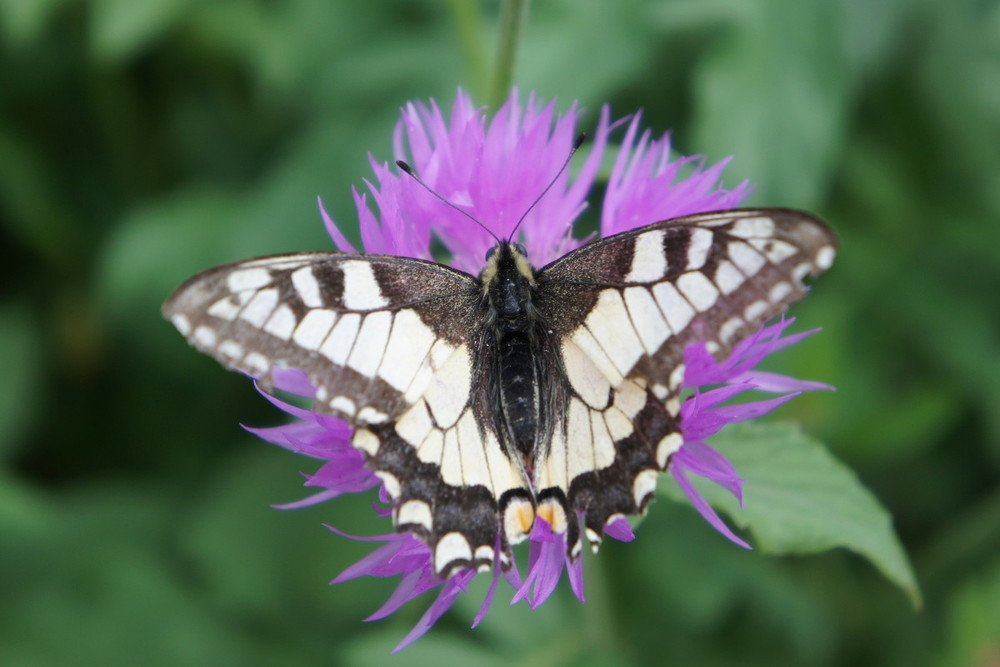
\includegraphics[width=0.95\textwidth]{FLY1000.jpg}
\column{0.5\linewidth}
\center
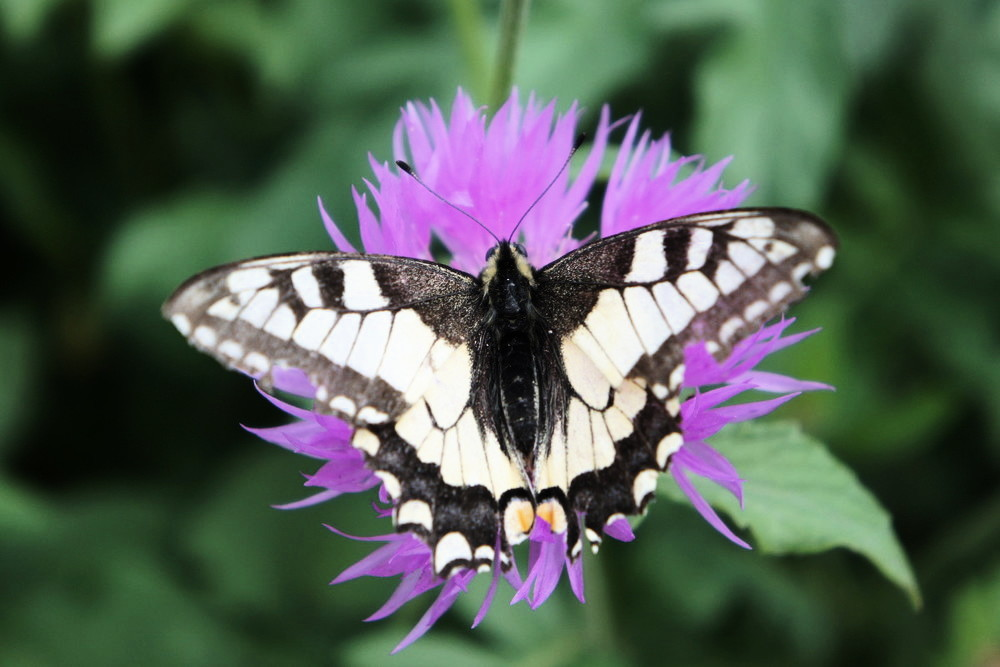
\includegraphics[width=0.95\textwidth]{FLY_contrast.jpg}
\end{columns}
\vfill
Уменьшение контраста:
\begin{lstlisting}
convert +contrast input.jpg output.jpg
\end{lstlisting}
\end{frame}


\begin{frame}[c, fragile]
\frametitle{Изменение яркости}
Увеличение яркости (от исходного значения 100):
\begin{lstlisting}
convert input.jpg -modulate 150 output.jpg
\end{lstlisting}
\begin{columns}
\column{0.5\linewidth}
\center
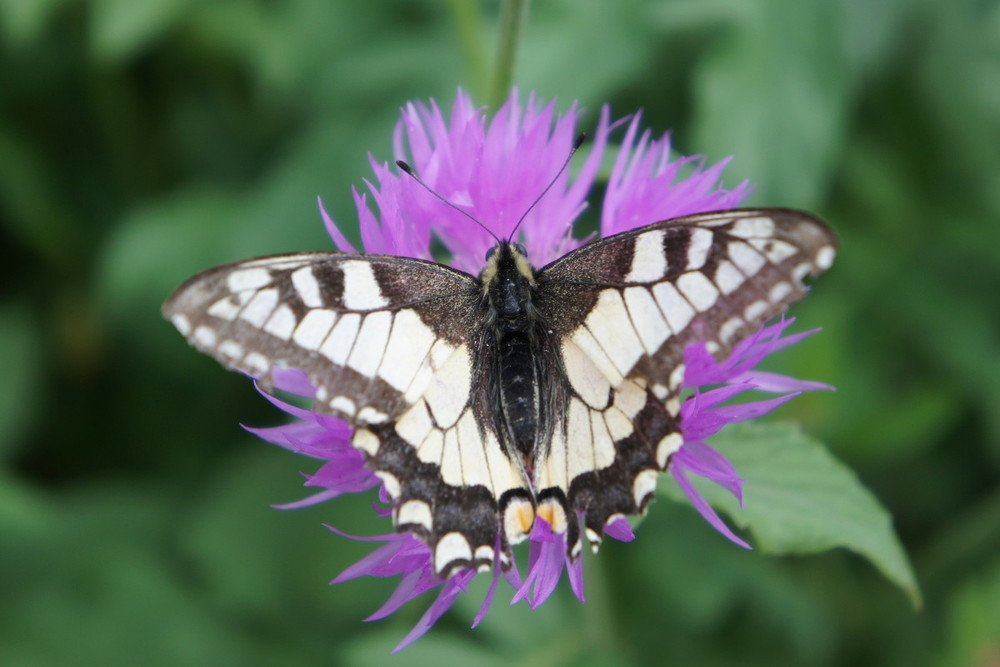
\includegraphics[width=0.95\textwidth]{FLY1000.jpg}
\column{0.5\linewidth}
\center
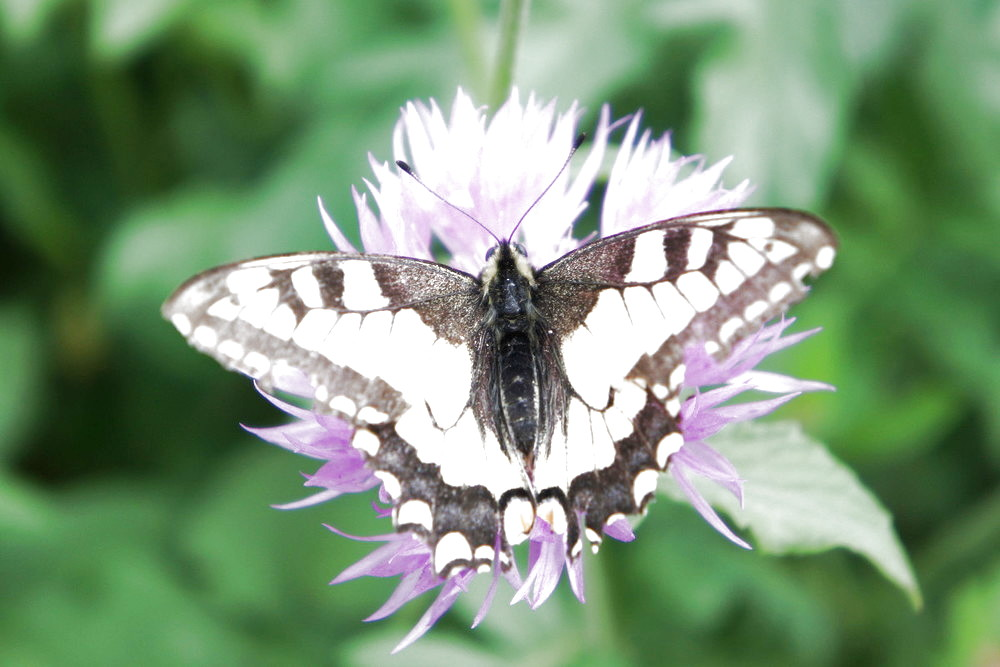
\includegraphics[width=0.95\textwidth]{FLY_modulate_150.jpg}
\end{columns}
\vfill
Уменьшение яркости:
\begin{lstlisting}
convert input.jpg -modulate 50 output.jpg
\end{lstlisting}
\end{frame}


\begin{frame}[c, fragile]
\frametitle{Изменение насыщенности}
Увеличение насыщенности (второй параметр \emph{-modulate}):
\begin{lstlisting}
convert input.jpg -modulate 130,150 output.jpg
\end{lstlisting}
\begin{columns}
\column{0.5\linewidth}
\center
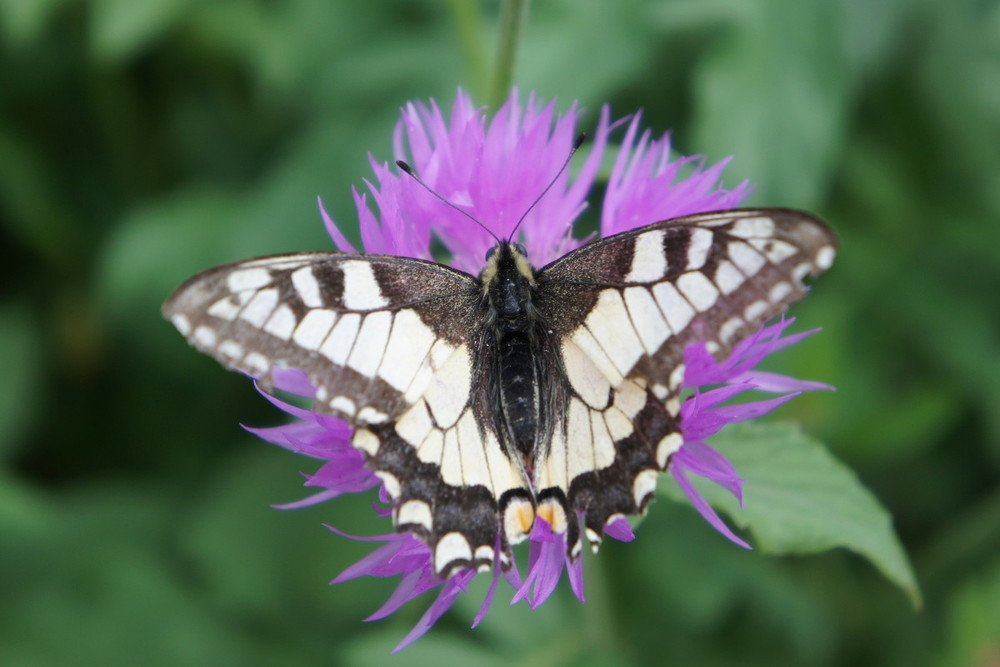
\includegraphics[width=0.95\textwidth]{FLY1000.jpg}
\column{0.5\linewidth}
\center
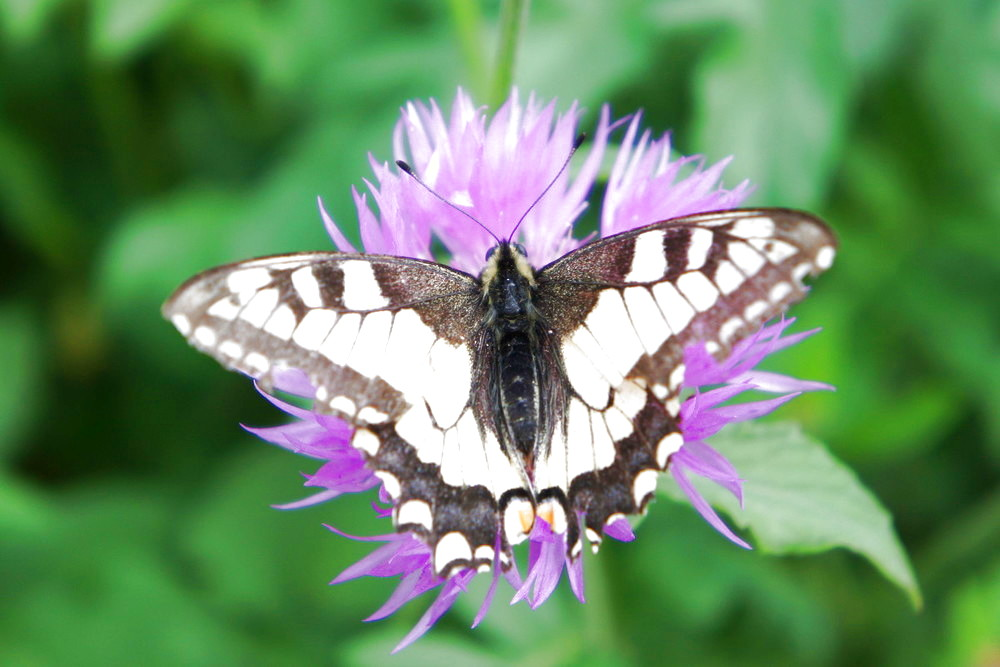
\includegraphics[width=0.95\textwidth]{FLY_modulate_130_150.jpg}
\end{columns}
\vfill
Градации серого:
\begin{lstlisting}
convert input.jpg -modulate 50,0 output.jpg
\end{lstlisting}
\end{frame}

\begin{frame}[c, fragile]
\frametitle{Изображение в градациях серого}
\begin{lstlisting}
convert image1.jpg -colorspace gray image2.jpg
\end{lstlisting}
\begin{columns}
\column{0.5\linewidth}
\center
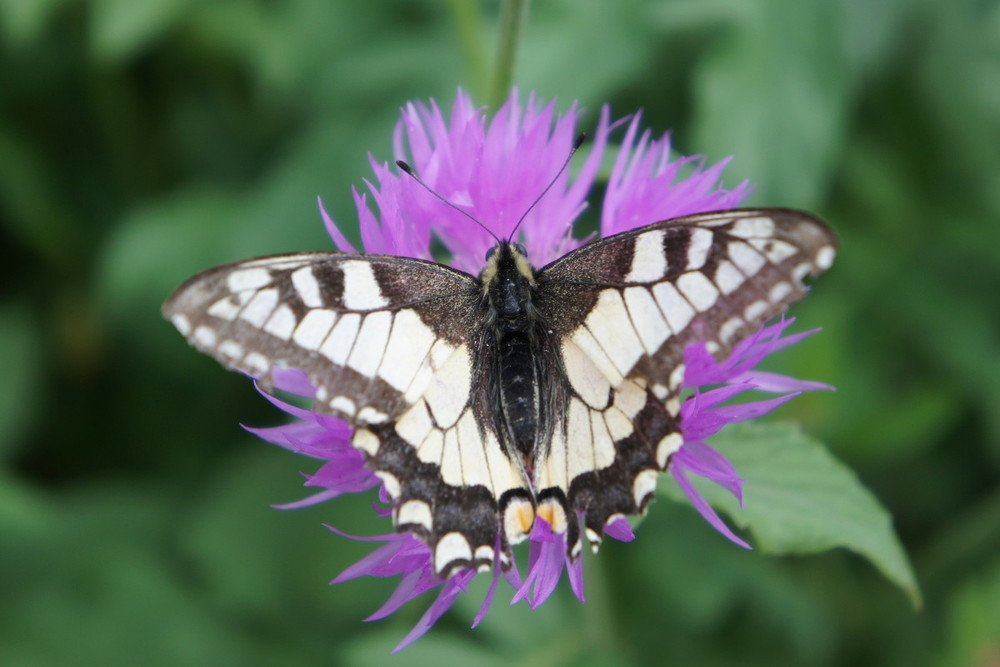
\includegraphics[width=0.95\textwidth]{FLY1000.jpg}
\column{0.5\linewidth}
\center
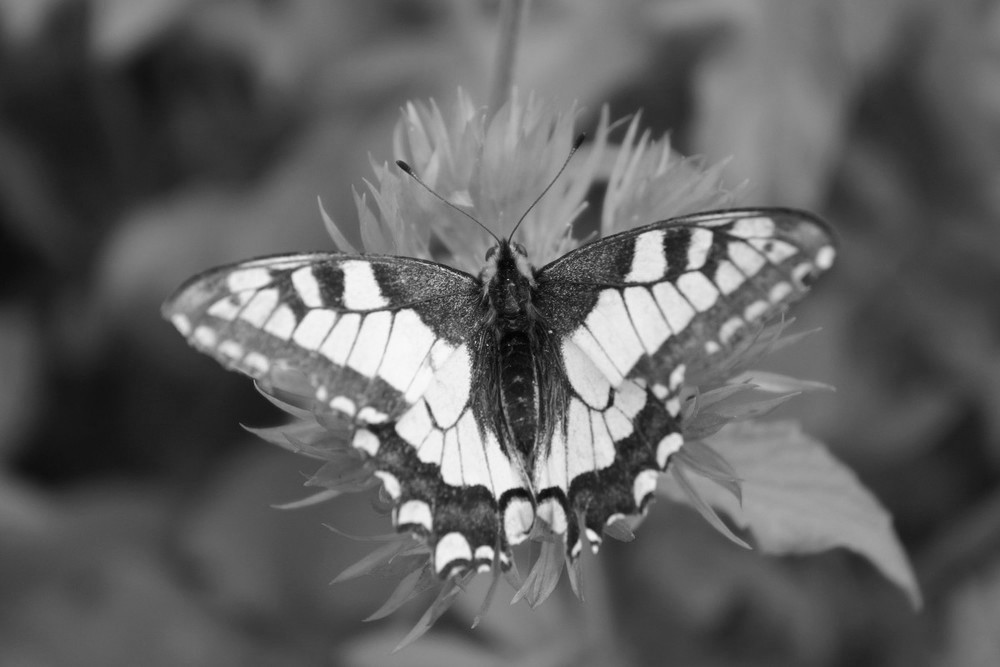
\includegraphics[width=0.95\textwidth]{FLY1000_grayscale.jpg}
\end{columns}
\end{frame}


\begin{frame}[c, fragile]
\frametitle{Негатив}
\begin{lstlisting}
convert image1.jpg -negate image2.jpg
\end{lstlisting}
\begin{columns}
\column{0.5\linewidth}
\center
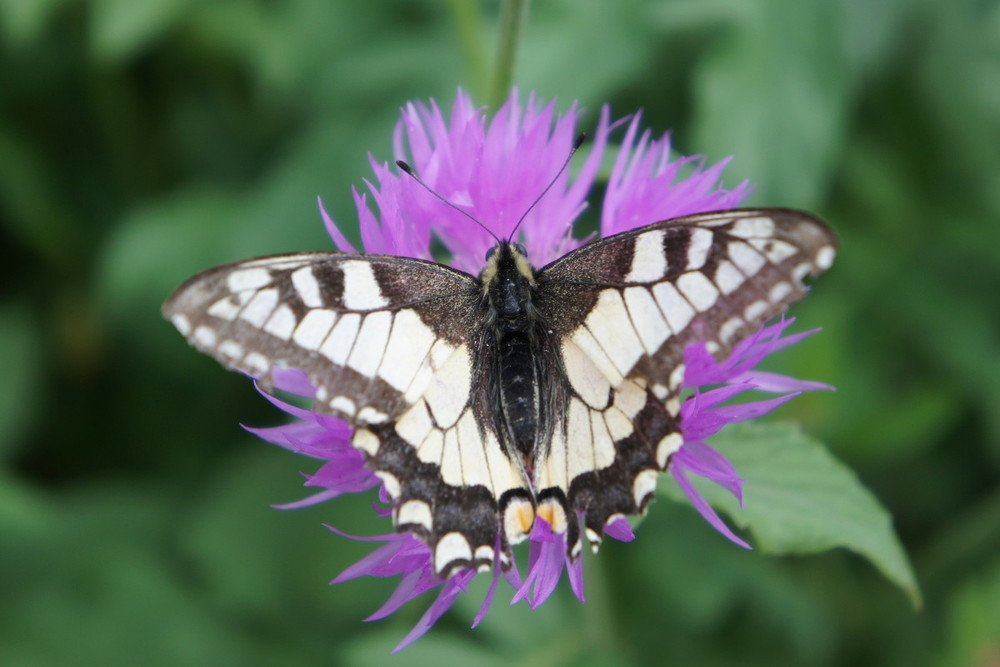
\includegraphics[width=0.95\textwidth]{FLY1000.jpg}
\column{0.5\linewidth}
\center
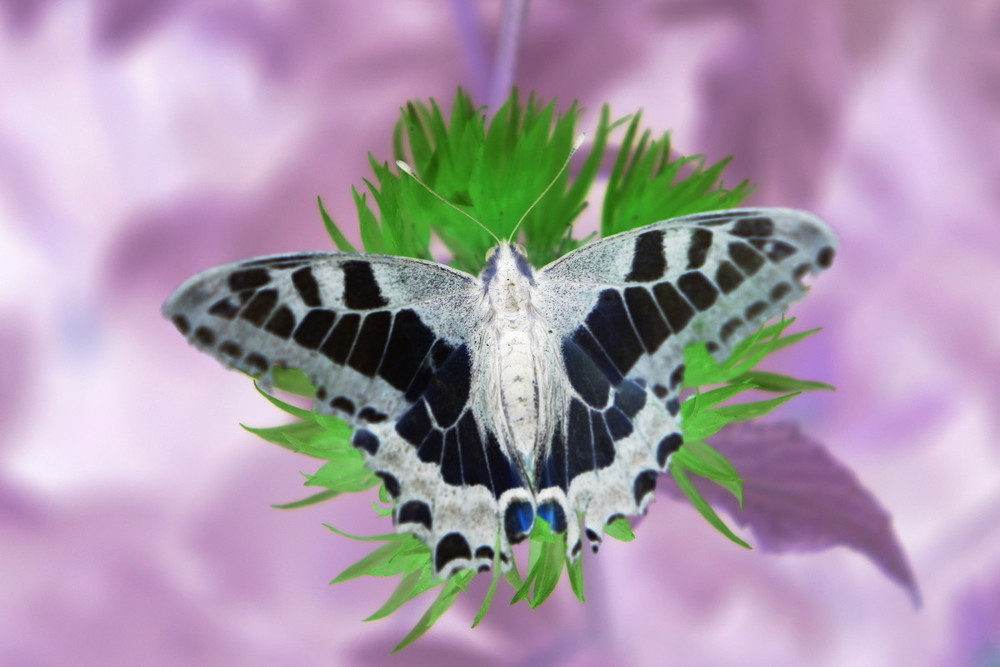
\includegraphics[width=0.95\textwidth]{FLY_negate.jpg}
\end{columns}
\end{frame}


\begin{frame}[c, fragile]
\frametitle{Сепия}
\begin{lstlisting}
convert image1.jpg -sepia-tone 55% image2.jpg
\end{lstlisting}
\begin{columns}
\column{0.5\linewidth}
\center
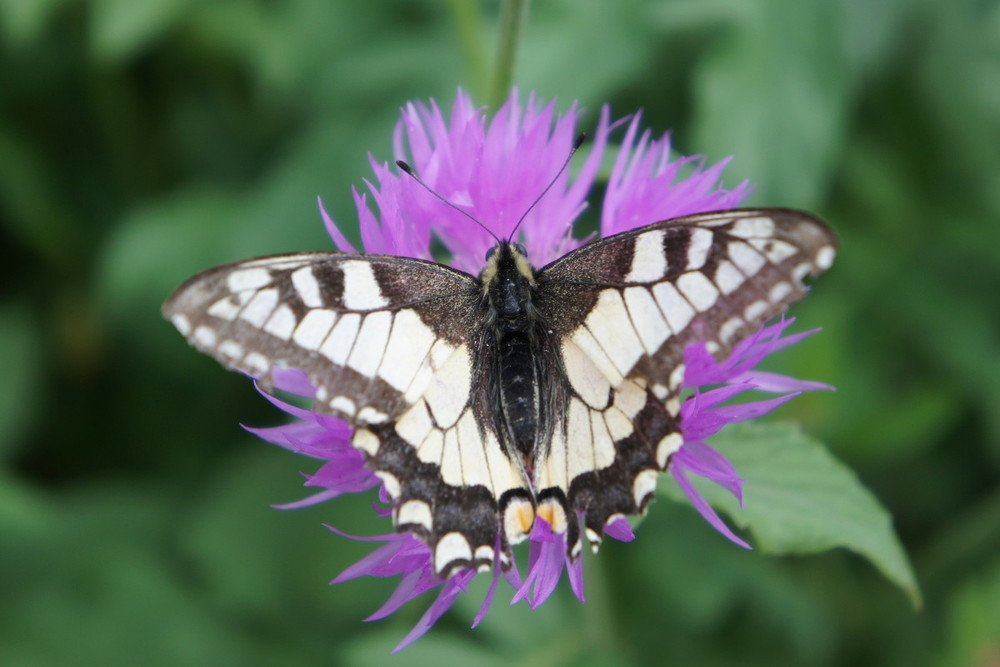
\includegraphics[width=0.95\textwidth]{FLY1000.jpg}
\column{0.5\linewidth}
\center 
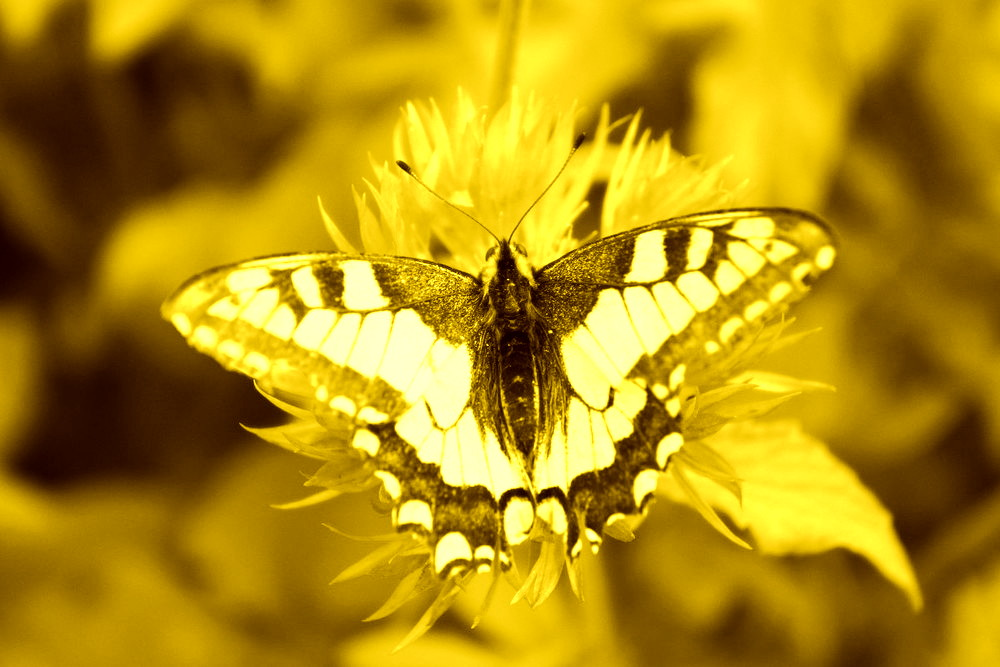
\includegraphics[width=0.95\textwidth]{FLY_sepia.jpg}
\end{columns}
\end{frame}

\begin{frame}[c, fragile]
\frametitle{Кадрирование}
Для обрезки изображения используется опция \emph{-shave dx,dy}. Срезка слева и справа по 150 точек, снизу и сверху -- 0:
\begin{lstlisting}
convert image1.jpg -shave 150x0 image2.jpg 
\end{lstlisting}
\end{frame}

\begin{frame}[c, fragile]
\frametitle{Кадрирование}
\begin{lstlisting}
convert image1.jpg -shave 150x20 image2.jpg 
\end{lstlisting}
\begin{columns}
\column{0.5\linewidth}
\center
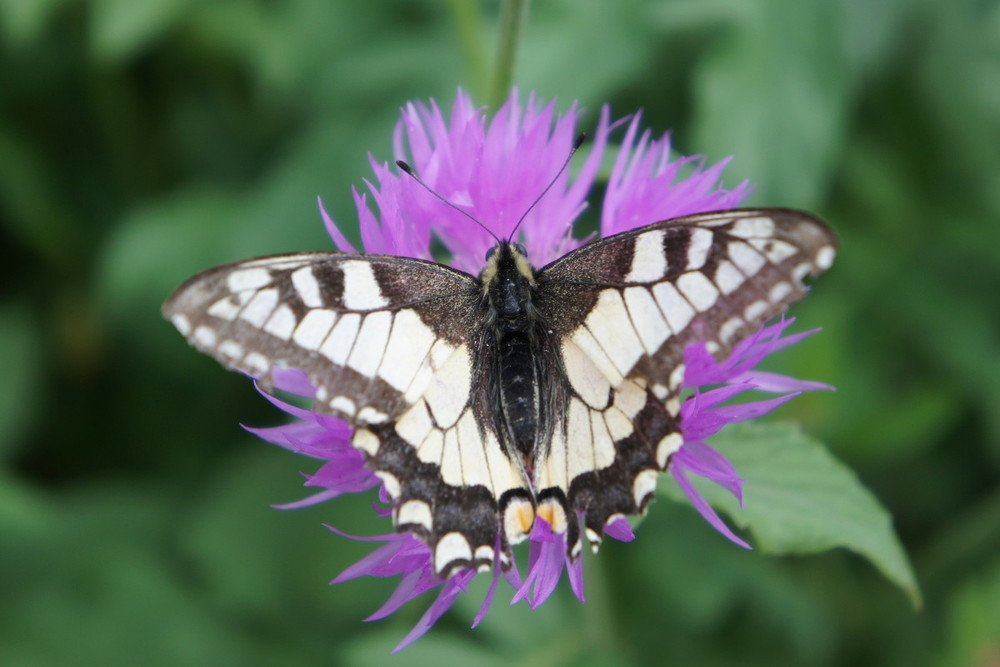
\includegraphics[width=0.95\textwidth]{FLY1000.jpg}
\column{0.5\linewidth}
\center
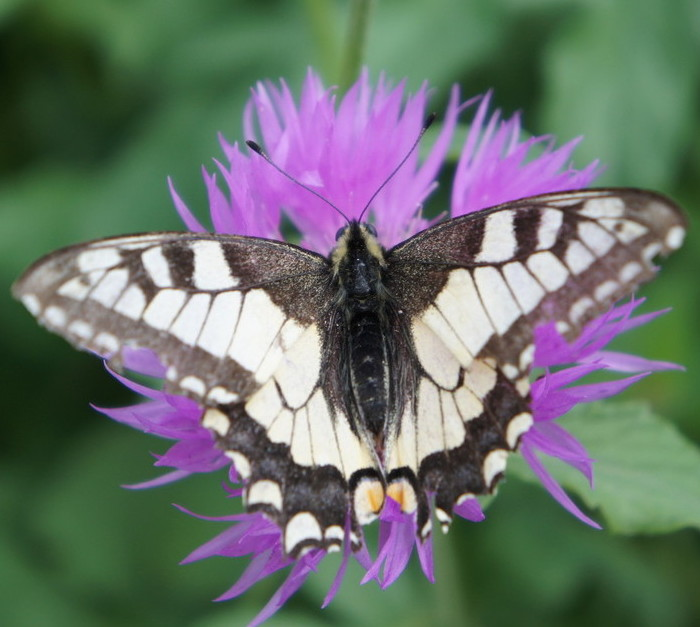
\includegraphics[width=0.67\textwidth]{FLY1000_shaved.jpg}
\end{columns}
\end{frame}

\begin{frame}[c, fragile]
\frametitle{Кадрирование}
\begin{lstlisting}
convert FLY.jpg -crop 200x200+150+250 FLY_crop.jpg
\end{lstlisting}
\begin{columns}
\column{0.5\linewidth}
\center
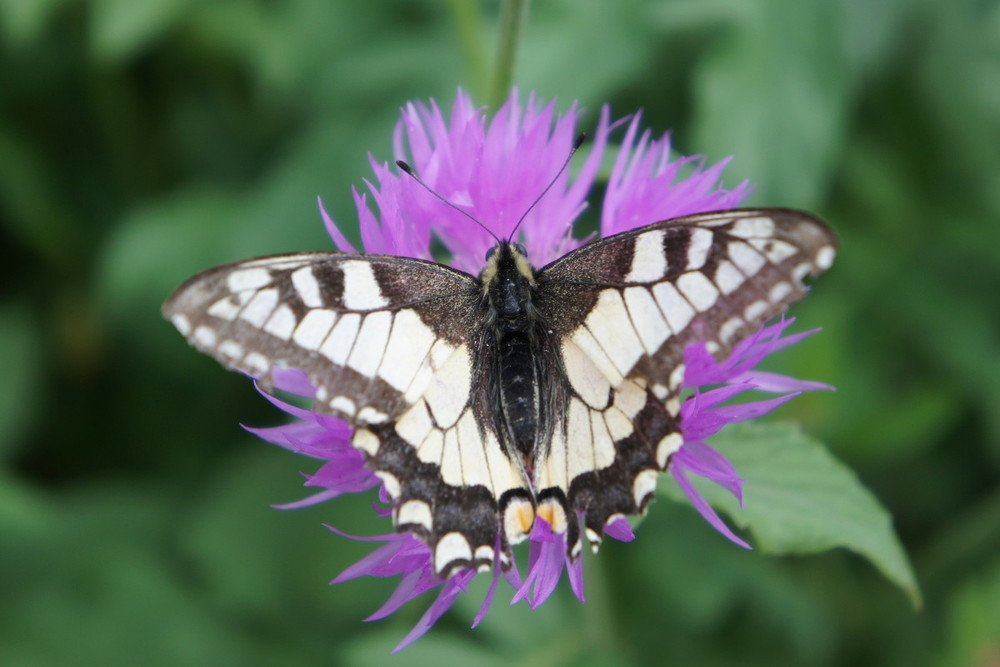
\includegraphics[width=0.95\textwidth]{FLY1000.jpg}
\column{0.5\linewidth}
\center
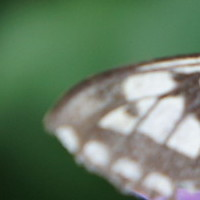
\includegraphics[width=0.65\textwidth]{FLY_crop.jpg}
\end{columns}
Вырезать фрагмент 200 на 200 точек, смещённый на 150 точек по горизонтали и 250 по вертикали относительно верхнего левого угла (начало координат изображения). 
\end{frame}

\begin{frame}[c, fragile]
\frametitle{Аннотация}
Подпись в левом верхнем углу (0,0) с отступом (полем) 10 по горизонтали и 10 по вертикали:
\begin{lstlisting}
convert image.jpg -annotate 0x0+10+10 
        "www.mypage.ru" image_annotated.jpg
\end{lstlisting}
{\centering
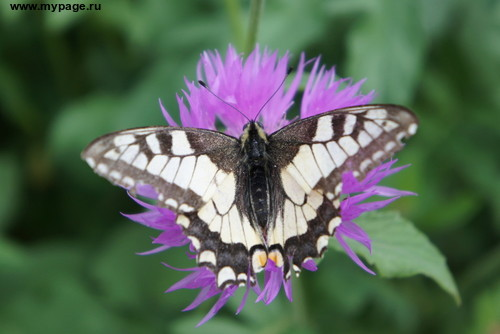
\includegraphics[width=0.6\textwidth]{FLY_annotated1.jpg}
}
\end{frame}

\begin{frame}[c, fragile]
\frametitle{Аннотация. Цвет текста}
\begin{lstlisting}
convert image.jpg -fill white 
        -annotate 0x0+10+10 "www.mypage.ru" 
        FLY_annotated.jpg
\end{lstlisting}
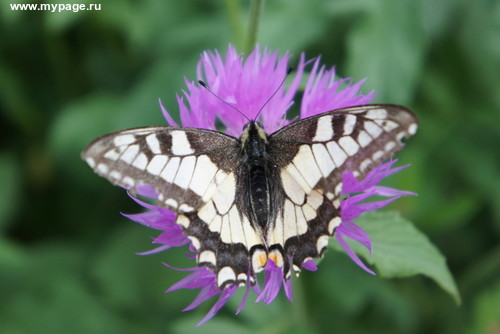
\includegraphics[width=0.6\textwidth]{FLY_annotated2.jpg}
\end{frame}

\begin{frame}[c, fragile]
\frametitle{Аннотация. Размер текста}
\begin{lstlisting}
convert image.jpg -fill white -pointsize 20
        -annotate 0x0+20+20 "www.mypage.ru" 
        FLY_annotated.jpg
\end{lstlisting}
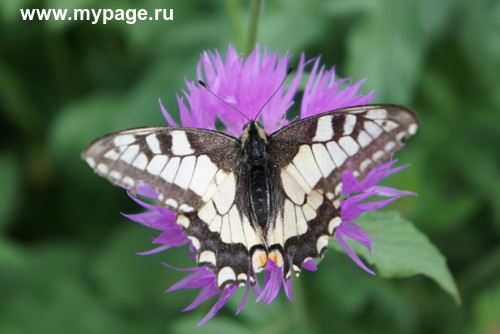
\includegraphics[width=0.6\textwidth]{FLY_annotated3.jpg}
\end{frame}

\begin{frame}[c, fragile]
\frametitle{Аннотация. Шрифт}
\begin{lstlisting}
convert image.jpg -fill white -pointsize 20
        -font "Comic Sans MS Bold.ttf"
        -annotate 0x0+20+20 "www.mypage.ru" 
        FLY_annotated.jpg
\end{lstlisting}
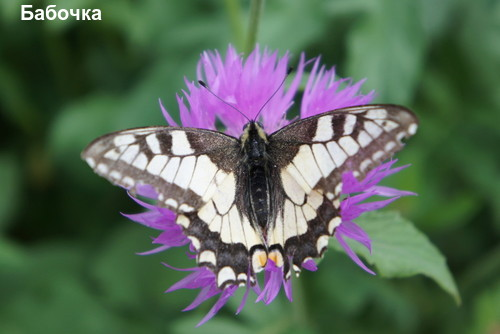
\includegraphics[width=0.6\textwidth]{FLY_annotated4.jpg}
\end{frame}


\begin{frame}[c, fragile]
\frametitle{Создание gif анимации}
\begin{itemize}
	\item Дана последовательность изображений (файлов).
	\item Необходимо создать анимированный gif из этих изображений-кадров с заданным интервалом времени между кадрами.
\begin{lstlisting}
convert -delay 30 p1.png p2.png p3.png 
        -loop 0 animation.gif
\end{lstlisting}	
  \code{-delay 30} -- интервал между кадрами 30 мс.\\
  \code{-loop 0} -- количество повторений (0 бесконечный цикл).
  \item Все изображения по шаблону имени
\begin{lstlisting}
convert -delay 30 page_*.png -loop 0 animation.gif
\end{lstlisting}  
\end{itemize}

\end{frame}


% =============================================================================
%
\section{FFMPEG}
%
% =============================================================================

\begin{frame}[c, fragile]
\frametitle{FFMPEG}
Консольный видеоредактор (видеоредактор командной строки), предназначенный для преобразования файлов. Основные утилиты:
\begin{itemize}
\item \emph{ffmpeg} -- программа для преобразования и редактирования видеофайлов
\item \emph{ffplay} -- видеоплеер
\item \emph{ffprobe} -- программа для извлечения информации о видеофайле
\end{itemize}
\end{frame}

\begin{frame}[c, fragile]
\frametitle{Варианты использования}
\begin{itemize}
	\item Преобразование видеофайла из одного формата в другой (mp4-wmv, mp4-webm, ...)
	\item Изменение размера видеоизображения
	\item Изменение частоты кадров
	\item Монтаж (извлечение фрагментов видеопотока)
	\item Создание анимированного gif из видеофайла
	\item Добавление текста на видеоизображение
\end{itemize}
\end{frame}

\begin{frame}[t]
\frametitle{Установка}
\url{https://www.ffmpeg.org/}
\centering
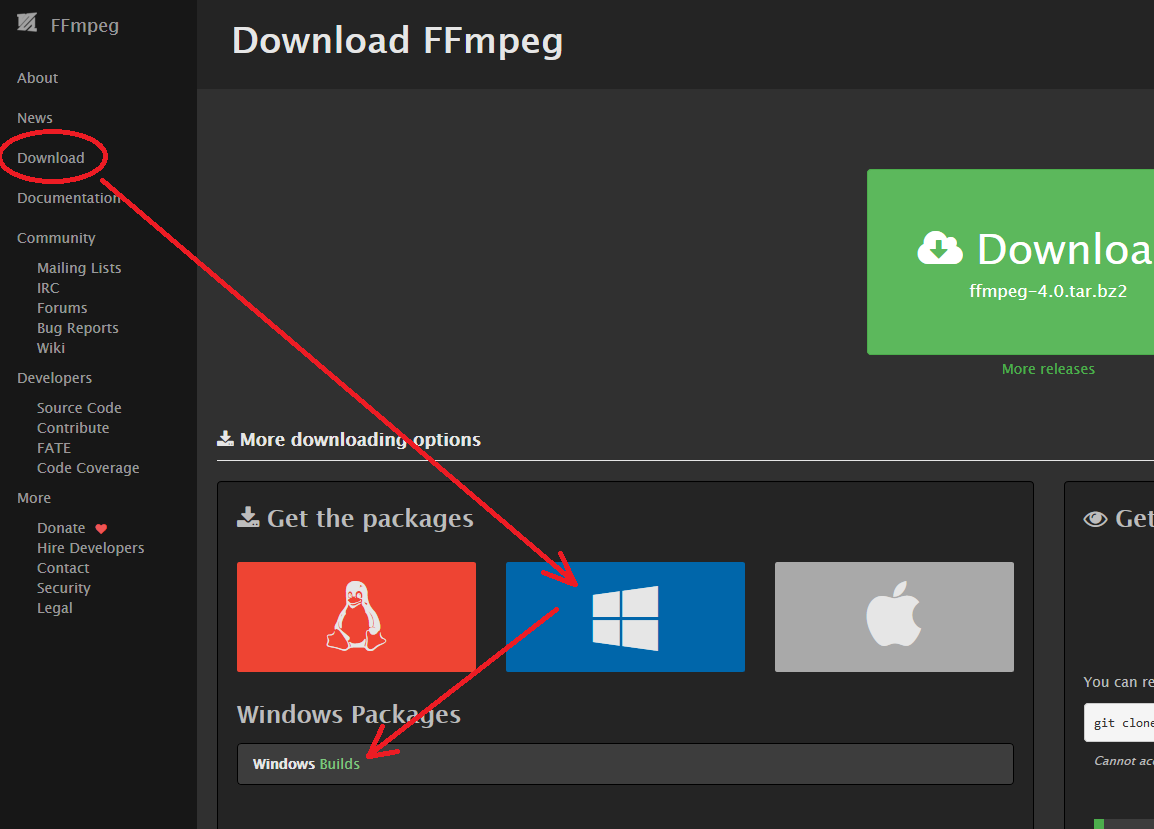
\includegraphics[width=0.95\textwidth]{ffmpeg_install_1.png}
\end{frame}


\begin{frame}[t]
\frametitle{Установка}
\url{https://ffmpeg.zeranoe.com/builds/}
\centering
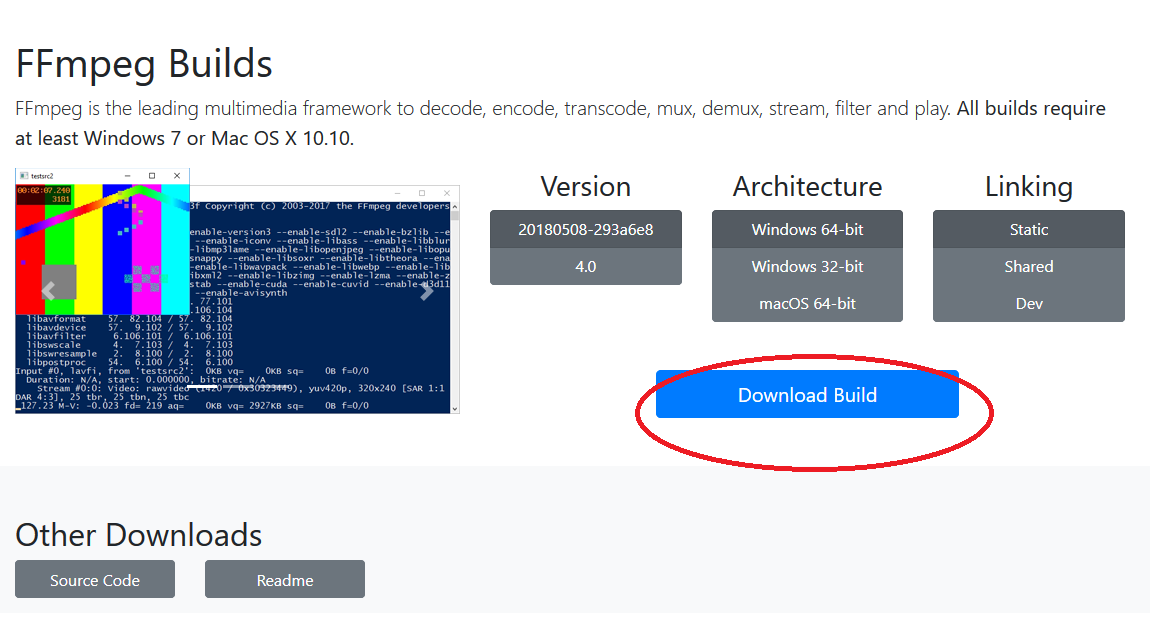
\includegraphics[width=0.95\textwidth]{ffmpeg_install_2.png}
\end{frame}

\begin{frame}[c, fragile]
\frametitle{Формат запуска программы}
\begin{lstlisting}
ffmpeg .1. .2. -i input_file .3. output_file
\end{lstlisting}
\begin{itemize}
  \item .1. - глобальные опции
  \item .2. - опции для исходного файла
  \item .3. - опции для файла-результата  
\end{itemize}
\end{frame}


\begin{frame}[c, fragile]
\frametitle{Преобразование формата}
Преобразование видеофайла в формат Windows Media Video (*.wmv) для гарантированной работоспособности видеофайла в презентации PowerPoint:
\begin{lstlisting}
ffmpeg -i net.avi -b:v 4M -vcodec msmpeg4 
       -acodec wmav2 net.wmv
\end{lstlisting}
Без аудиодорожки
\begin{lstlisting}
ffmpeg -i net.avi -b:v 4M 
       -vcodec msmpeg4 -an net.wmv
\end{lstlisting}
\begin{itemize}
\item \emph{-b:v 4M} -- битрейт видеопотока (Мб/с)
\item \emph{-vcodec msmpeg4} -- тип сжатия видео (``codec'') Microsoft MPEG-4
\item \emph{-acodec wmav2} -- тип сжатия аудио Windows Media Audio
\end{itemize}
\end{frame}



\begin{frame}[c,fragile]
\frametitle{Типы сжатия}
\begin{itemize}
\item Качество видеофайла-результата определяется ``битрейтом'' и типом сжатия.
\item Чем выше битрейт видеопотока (\emph{-b:v}), тем выше качество результирующего файла.
\item Список поддерживаемых типов сжатия:
\begin{lstlisting}
ffmpeg -codecs
\end{lstlisting}  
или
\begin{lstlisting}
ffmpeg -encoders
\end{lstlisting}  
\end{itemize}
\end{frame}

\begin{frame}[c,fragile]
\frametitle{Совместимость}
\href{https://superuser.com/questions/859010/what-ffmpeg-command-line-produces-video-more-compatible-across-all-devices}{Перекодирование} для поддержки большинства устройств:
\begin{lstlisting}
ffmpeg -i input.avi 
       -c:v libx264 -crf 23 -profile:v baseline 
       -level 3.0 -pix_fmt yuv420p 
       -c:a aac -ac 2 -strict experimental -b:a 128k 
       -movflags faststart output.mp4
\end{lstlisting}
\emph{libx264} или MPEG-4 Part 10, Advanced Video Coding (MPEG-4 AVC) наиболее распространённый стандарт эффективного кодирования видео. Поддерживает разрешение до 8192 на 4320 точек.
\end{frame}


\begin{frame}[c, fragile]
\frametitle{Изменение размера и качества сжатия}
Для изменения размера изображения используется опция 
\emph{-s ШИРИНАxВЫСОТА}:
\begin{lstlisting}
ffmpeg -i net.avi -s 320x240 net_320x240.mp4
\end{lstlisting}  
Можно указать только один размер, а второй установить в -1. В этом случае неуказанный размер (-1) будет  вычисляться:
\begin{lstlisting}
ffmpeg -i net.avi -s 320x240 net_320x240.mp4
\end{lstlisting}  
\end{frame}

\begin{frame}[c, fragile]
\frametitle{Фрагменты}
Вырезать из видеофайла input.wmv фрагмент с 30 секунды продолжительностью 10 секунд:
\begin{lstlisting}
ffmpeg -ss 00:00:30.0 -i input.wmv 
       -c copy -t 00:00:10.0 output.wmv
\end{lstlisting}
\begin{itemize}
\item \emph{-ss 00:00:30} -- с 30 секунды
\item \emph{-t 00:00:10.0} -- продолжительность 10 секунд
\item \emph{-с copy} -- копировать видео и аудиопотоки (без ``пережатия'')
\end{itemize}
\end{frame}

\begin{frame}[c, fragile]
\frametitle{Склейка}
Для склейки нескольких видеофайлов, закодированных в одном формате, необходимо создать текстовый файл
\begin{block}{my-video.txt}
\begin{lstlisting}
file 'file1.avi'
file 'file2.avi'
file 'file3.avi'
\end{lstlisting}
\end{block}
\begin{lstlisting}
ffmpeg -f concat -i my-video.txt -c copy output.avi
\end{lstlisting}
\end{frame}

\begin{frame}[c, fragile]
\frametitle{Извлечение одного кадра из видеофайла}
\begin{lstlisting}
ffmpeg -ss 00:00:01 -i video.avi -vframes 1 
       video_frame.png
\end{lstlisting}
\end{frame}


\begin{frame}[c, fragile]
\frametitle{Извлечение нескольких кадров из видеофайла}
\begin{itemize}
  \item Исходный видеофайл \code{net\_case\_1.avi}
  \item Необходимо получить изображения (``стоп-кадры'') с шагом 1 c.
\end{itemize}
\end{frame}

\begin{frame}[c, fragile]
\frametitle{Извлечение кадров}
\begin{lstlisting}
ffmpeg -i net_case_1.avi -vf fps=1 case_1_%3d.png
\end{lstlisting}
\begin{center}
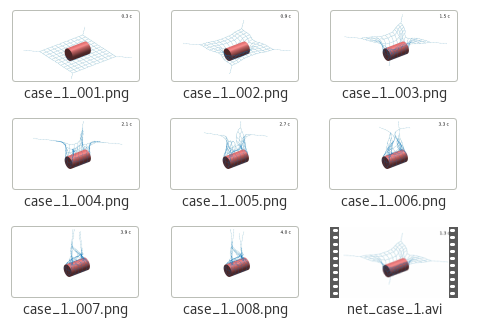
\includegraphics[width=0.9\textwidth]{montage_gallery.png}
\end{center}
\end{frame}


\begin{frame}[c, fragile]
\frametitle{Построение ``галереи''}
\begin{lstlisting}
montage case_1_*.png -tile 2x -geometry +1+1 gal1.png
\end{lstlisting}
\begin{center}
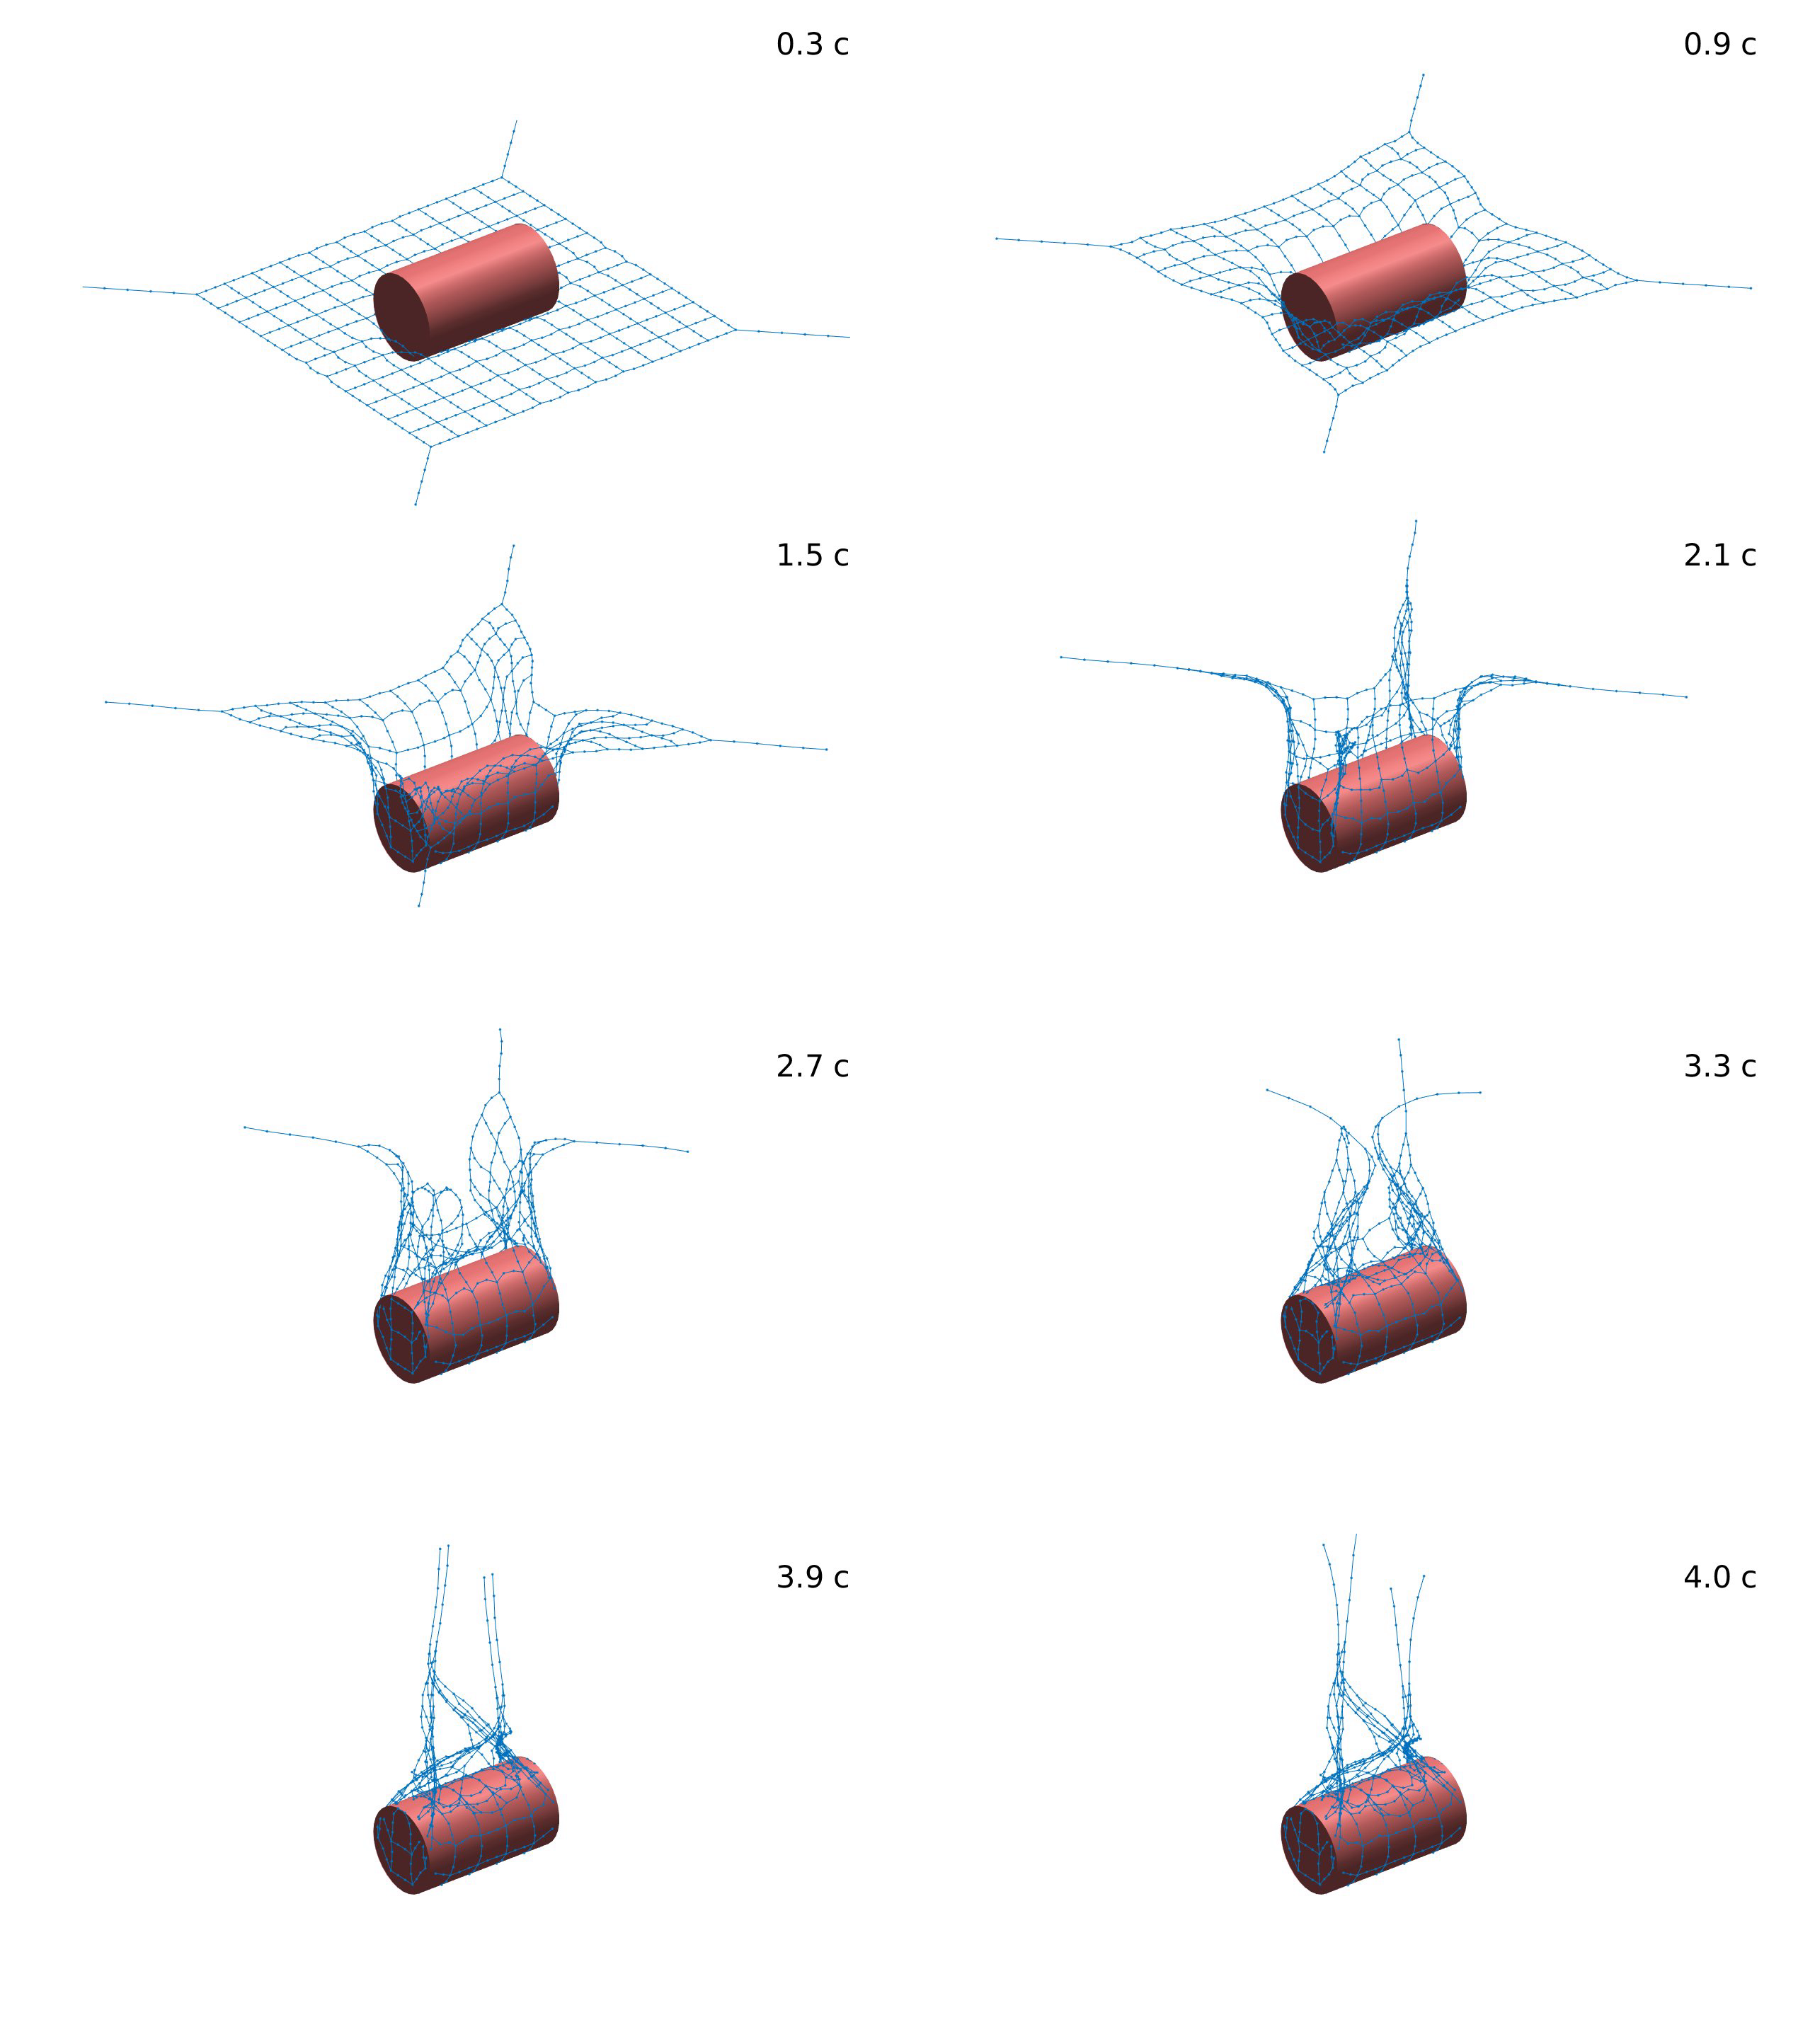
\includegraphics[width=0.45\textwidth]{gal1.png}
\end{center}
\end{frame}


\begin{frame}[c, fragile]
\frametitle{Построение ``галереи''}
\begin{lstlisting}
montage case_1_*.png -border 2x2 
        -bordercolor gray  -tile x2 
        -geometry +10+10 gal2.png
\end{lstlisting}
\begin{center}
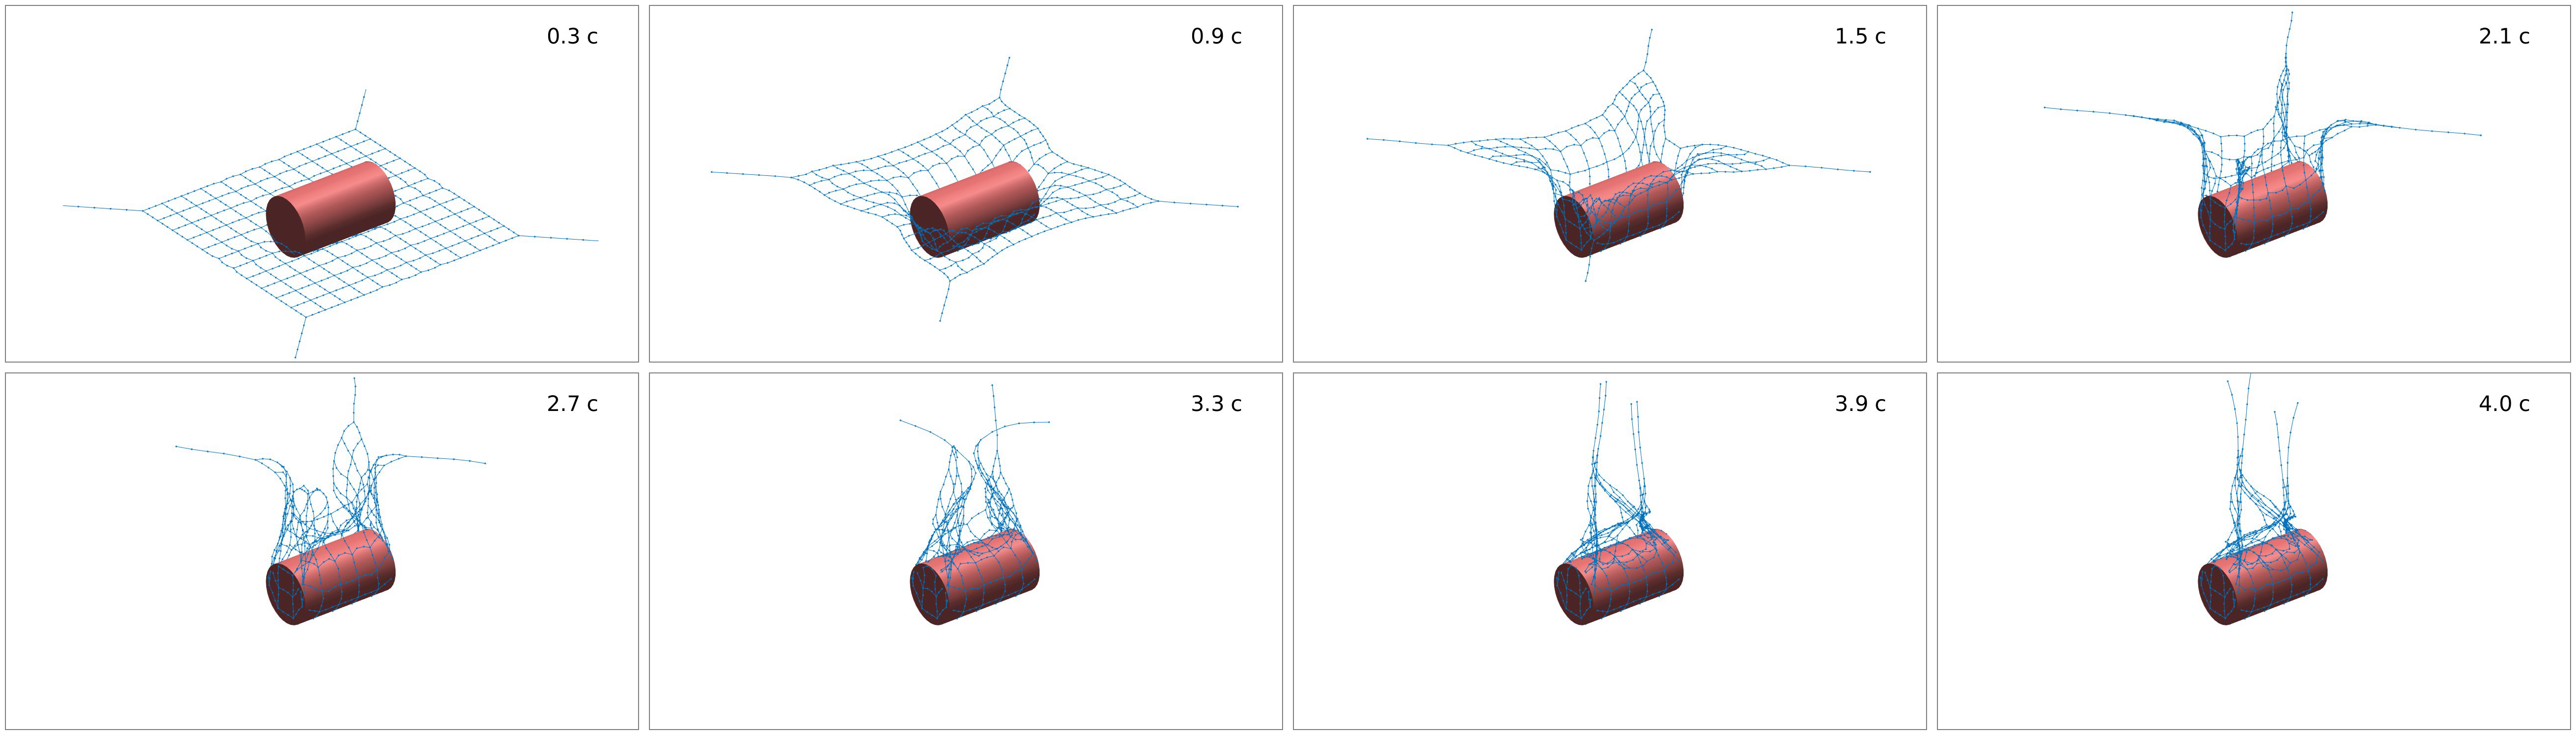
\includegraphics[width=1\textwidth]{gal2.png}
\end{center}
\end{frame}


\begin{frame}[c, fragile]
\frametitle{Построение ``галереи'' в рамках}
\begin{lstlisting}
montage case_1_001.png case_1_008.png 
        -border 2x2 -bordercolor gray 
        -tile 2x -geometry -2-2 gal3.png
\end{lstlisting}
\begin{center}
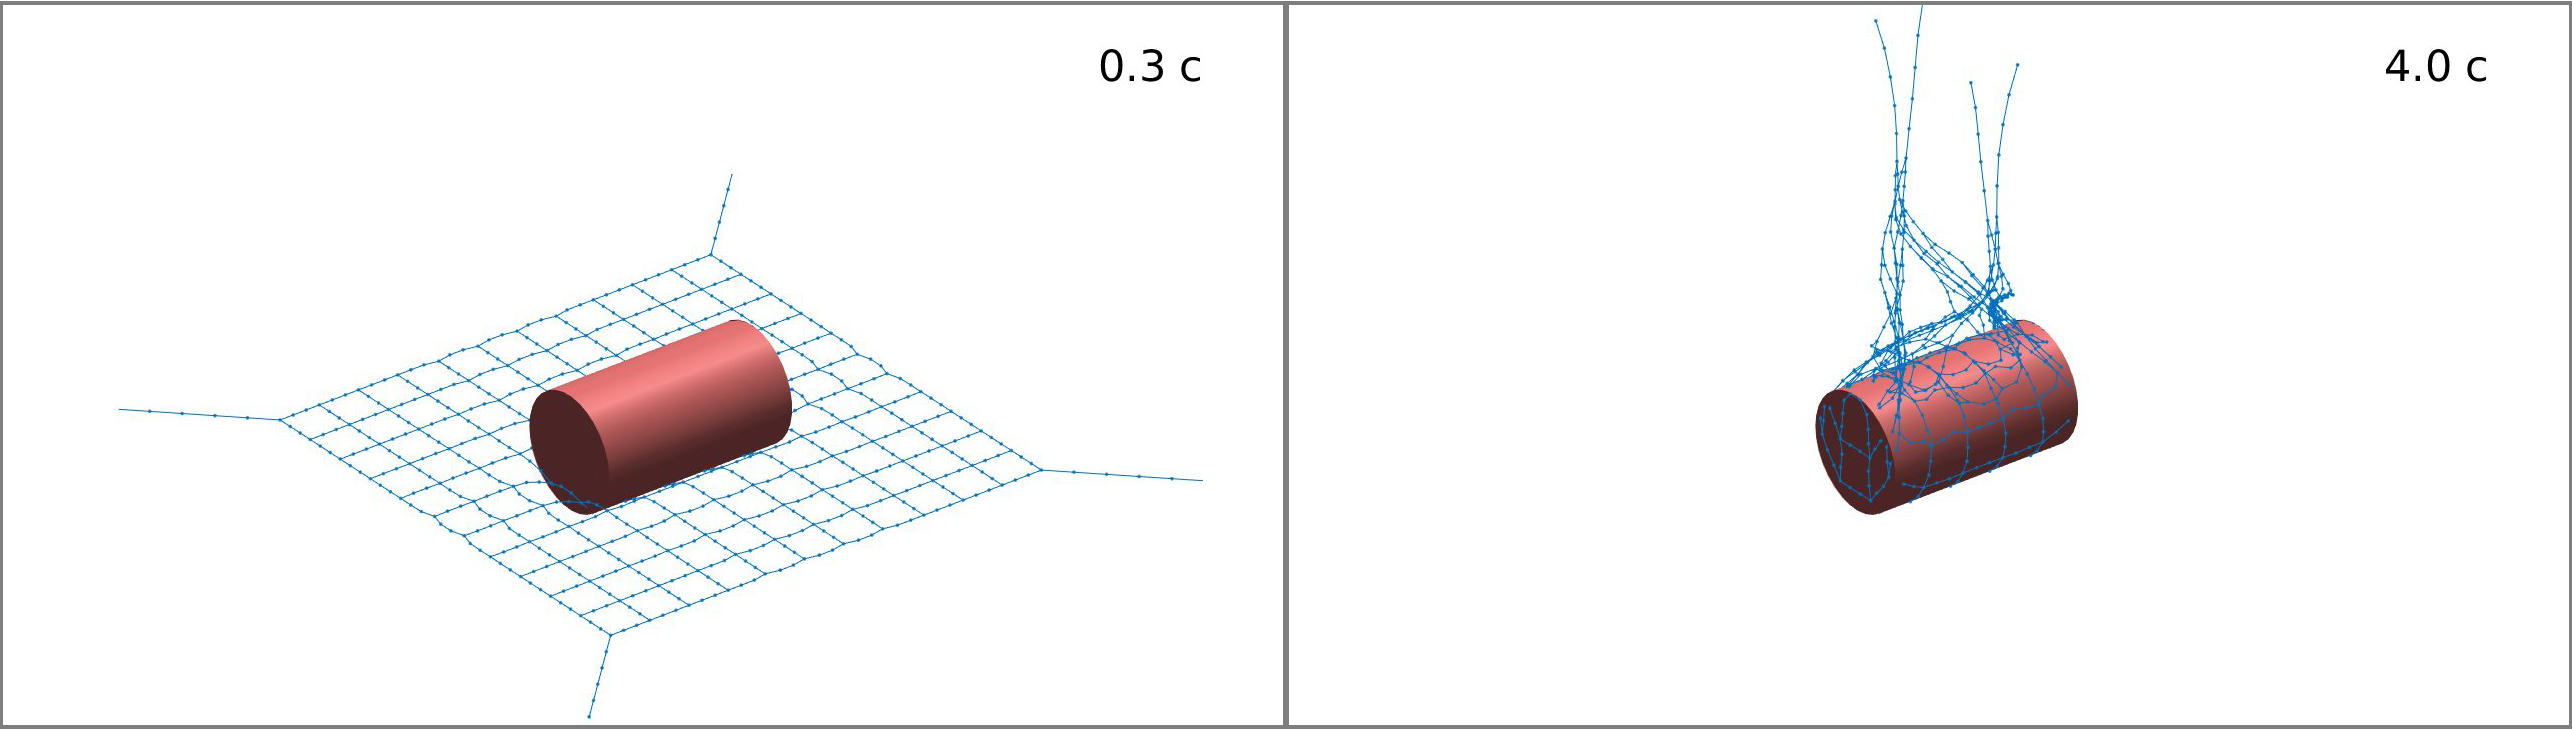
\includegraphics[width=1\textwidth]{gal3.png}
\end{center}
\end{frame}

\begin{frame}[c,fragile]
\frametitle{Видеопрезентация из изображений}
\begin{itemize}
\item есть несколько изображений p01.png, p02.png, p03.png, ...
\item требуется создать видеофайл продолжительностью 5 секунд  
\item каждые 5 секунд должно появляться новое изображение
\item частота кадров видеофайла 30 кадров в секунду
\end{itemize}
\begin{lstlisting}
ffmpeg -r 1/5 -i p%2d.png -c:v libx264 -r 30 
       -y -pix_fmt yuv420p slide_show.mp4 
\end{lstlisting}
\end{frame}

\begin{frame}[c,fragile]
\frametitle{Добавление аннотации}
\begin{lstlisting}
ffmpeg -i net.avi 
       -vf "drawtext=text='Net capture':
       fontcolor=black@0.6:fontsize=18:box=1:
       boxcolor=black@0.0:x=5:y=5" 
       -b:v 4M -y net_annotated.avi 
\end{lstlisting}  
\begin{columns}
\column{0.5\linewidth} 
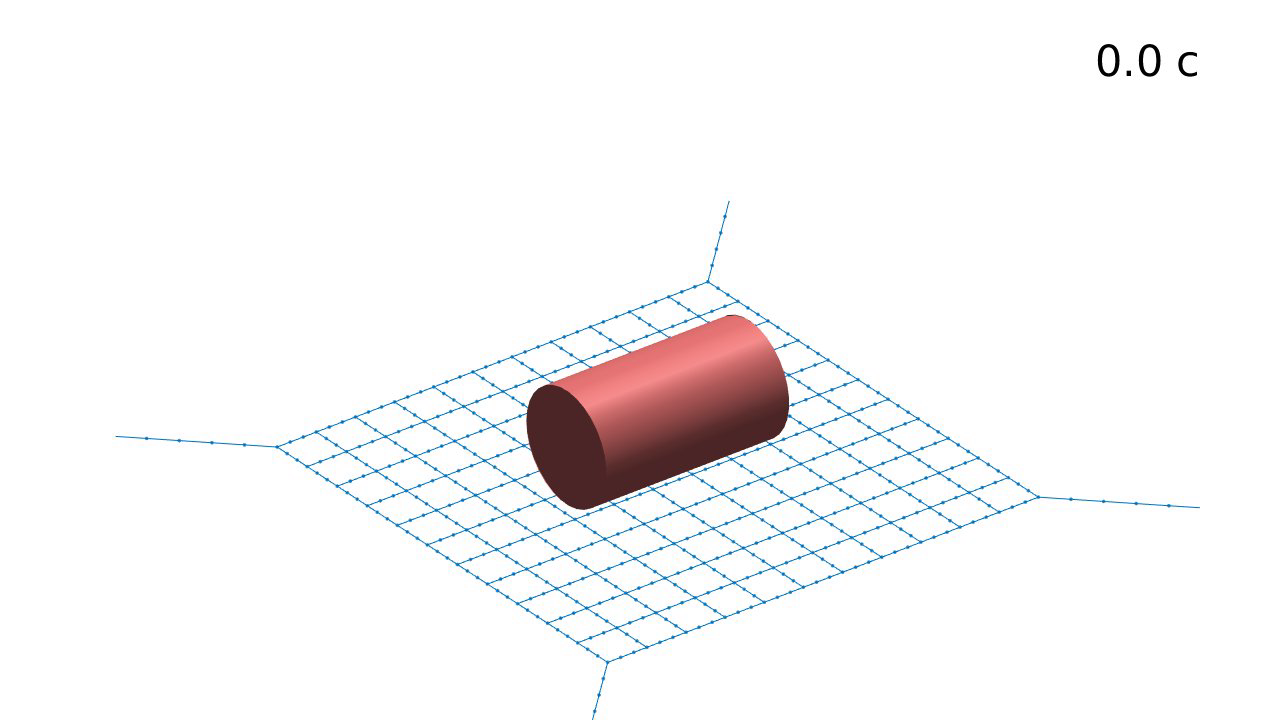
\includegraphics[width=1\textwidth]{net_wo_annotation.png}
\column{0.5\linewidth}
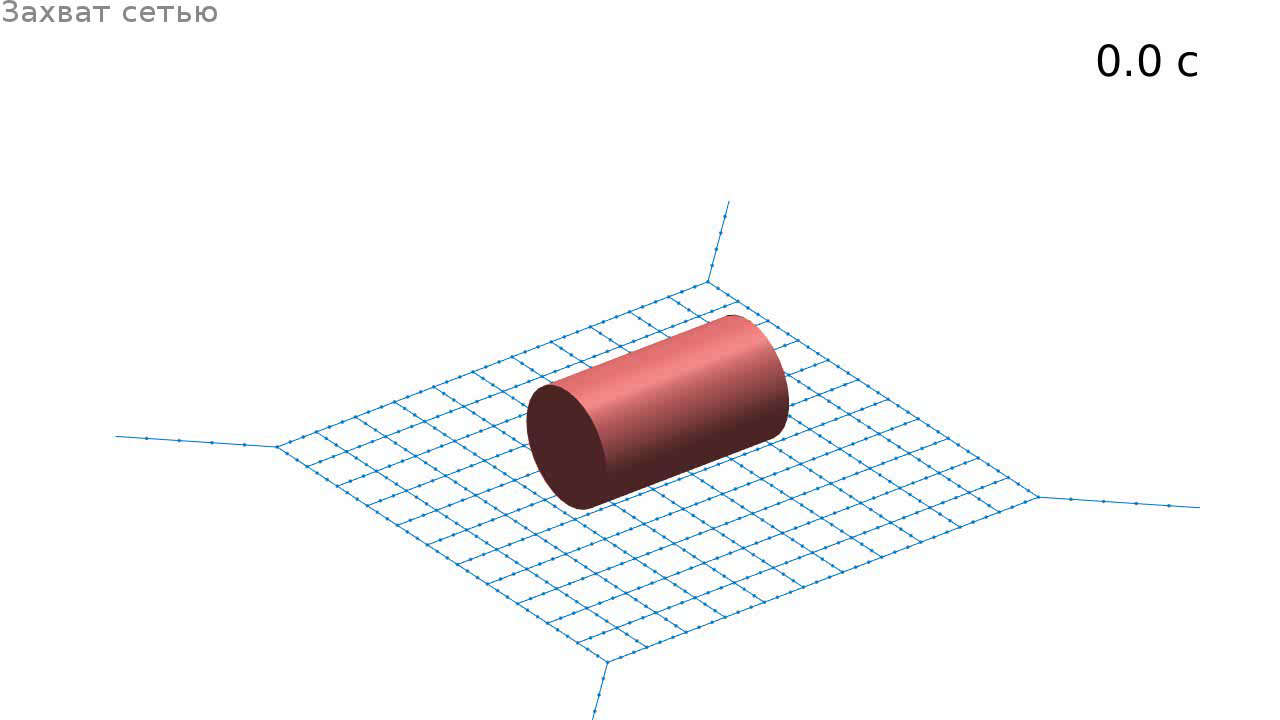
\includegraphics[width=1\textwidth]{net_with_annotation.png}
\end{columns}     
\end{frame}

\begin{frame}[c,fragile]
\frametitle{Анимированный gif из видеофайла}
\begin{lstlisting}
ffmpeg -i video.avi video.gif 
\end{lstlisting}
\begin{columns}
\column{0.5\linewidth}
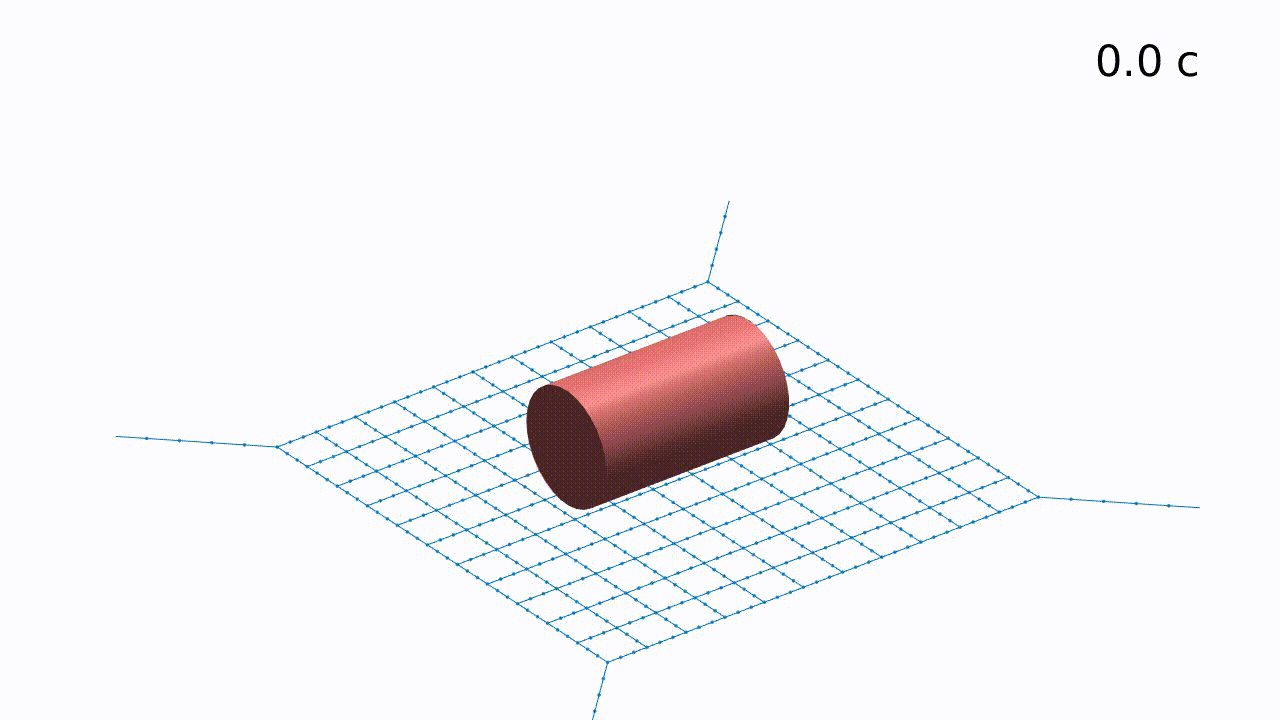
\includegraphics[width=1\textwidth]{net_gif.png}
\column{0.5\linewidth}
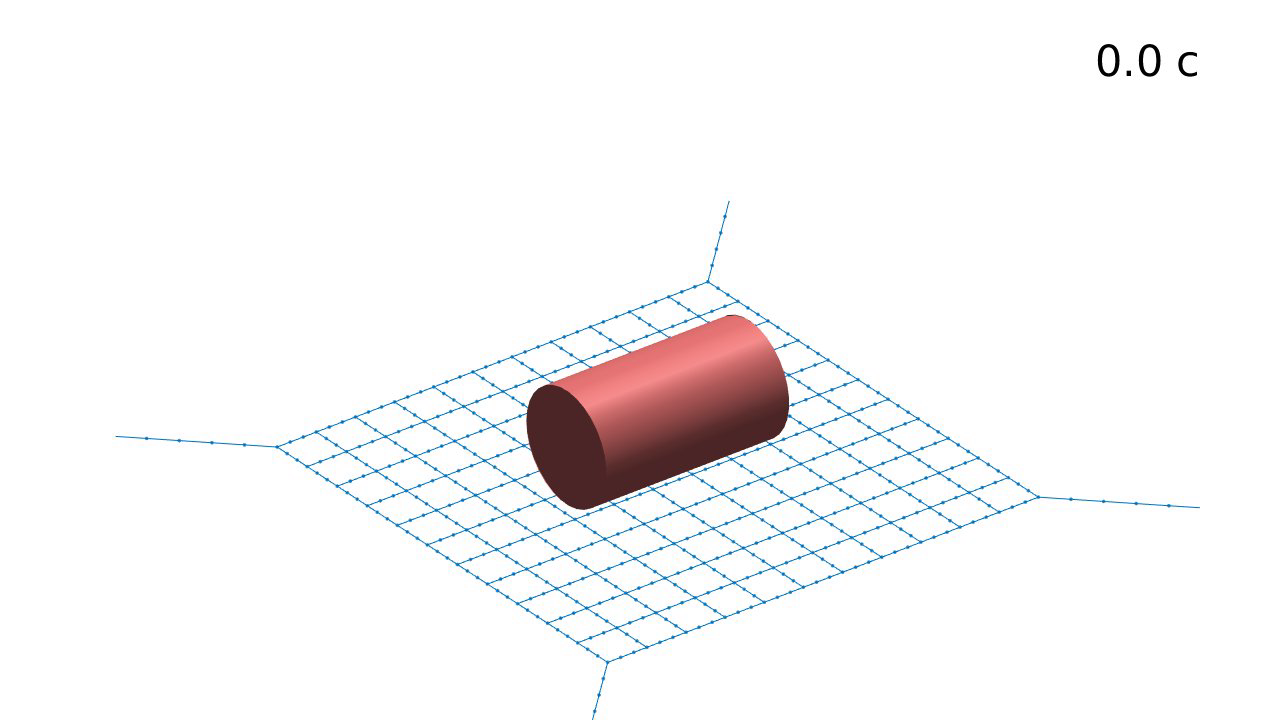
\includegraphics[width=1\textwidth]{net_0.png}
\end{columns}
\end{frame}


\begin{frame}[c]
\frametitle{Задание}
Используя анимацию движения механизма из курсовой работы по механике, построить галерею 2x3 из шести характерных изображений положений механизма.
\end{frame}

\begin{frame}[c]
\frametitle{Источники}
\begin{itemize}
	\item \url{https://www.imagemagick.org}	
	\item \url{http://najomi.org/_nix/imagemagick}
	\item \url{https://www.ffmpeg.org/}
	\item \url{https://habrahabr.ru/post/333664/}	
\end{itemize}	
\end{frame}

\end{document}
